\documentclass[aps,prd,twocolumn,superscriptaddress,nofootinbib,floatfix]{revtex4-2}

\usepackage{graphicx}
\usepackage{amsmath}
\usepackage{amssymb}
\usepackage{dcolumn}
\usepackage{bm}
\usepackage{hyperref}
\usepackage{xcolor}

% upright differentials
\newcommand{\dd}{\mathrm{d}}
\graphicspath{{figures/}}

\hypersetup{colorlinks=true,linkcolor=blue,citecolor=blue,urlcolor=blue}

\begin{document}

\title{Joint Cluster Number Counts and Masked Thermal Sunyaev-Zel'dovich Power Spectrum Analyses: Validation on Synthetic Skies and Application to the FLAMINGO Simulations}

\author{Licong Xu}
\email{lx256@cam.ac.uk}
\affiliation{Institute of Astronomy, University of Cambridge, Madingley Road, Cambridge CB3 0HA, UK}
\affiliation{Kavli Institute for Cosmology, University of Cambridge, Madingley Road, Cambridge CB3 0HA, UK}

\author{I\~nigo Zubeldia}
\affiliation{Institute of Astronomy, University of Cambridge, Madingley Road, Cambridge CB3 0HA, UK}
\affiliation{Kavli Institute for Cosmology, University of Cambridge, Madingley Road, Cambridge CB3 0HA, UK}
\affiliation{DAMTP, Centre for Mathematical Sciences, Wilberforce Road, Cambridge CB3 0WA, UK}

\author{Boris Bolliet}
\affiliation{Cavendish Astrophysics, University of Cambridge, Madingley Road, Cambridge CB3 0HA, UK}
\affiliation{Kavli Institute for Cosmology, University of Cambridge, Madingley Road, Cambridge CB3 0HA, UK}

\author{Anthony Challinor}
\affiliation{Institute of Astronomy, University of Cambridge, Madingley Road, Cambridge CB3 0HA, UK}
\affiliation{Kavli Institute for Cosmology, University of Cambridge, Madingley Road, Cambridge CB3 0HA, UK}
\affiliation{DAMTP, Centre for Mathematical Sciences, Wilberforce Road, Cambridge CB3 0WA, UK}

\date{\today}

\begin{abstract}
We present a self-consistent joint analysis of the thermal Sunyaev-Zel'dovich (tSZ) angular power spectrum and cluster number counts (CNC) in which clusters detected above a signal-to-noise threshold $q_{\mathrm{cat}}$ are masked from the power spectrum and used instead as the CNC sample, so that the two probes act on non-overlapping halo populations.
Using synthetic \textit{Planck}-like data from a halo-painting pipeline, we show that masking renders the binned bandpower distribution statistically Gaussian in every multipole bin, whereas the full-sky distribution is strongly skewed at $\ell \lesssim 100$.
In full MCMC analyses of the synthetic skies the joint CNC plus masked-tSZ combination yields $\sigma(\Omega_{\mathrm{m}}) = 0.008$, $\sigma(\sigma_8) = 0.009$, and $\sigma(F) = 0.003$ for the tSZ degeneracy combination $F \equiv \sigma_8 (\Omega_{\mathrm{m}}/B)^{0.40} (h/0.7)^{-0.21}$, factors of $1.4$ to $5$ tighter than any single probe; with foreground contamination the same gains persist at the factor $2$ to $4$ level, but the analysis is then limited by the modelling of the foreground residuals, whose most tSZ-degenerate template absorbs a $3.8\sigma$ amplitude bias.
We then apply the masking method to light-cone Compton-$y$ maps and halo catalogues from the FLAMINGO hydrodynamical simulations to investigate how the shape of the tSZ power spectrum changes as the most massive clusters are masked progressively, thereby isolating the contributions of different halo populations to the tSZ signal.
Progressive masking suppresses the spectrum in a strongly scale-dependent way (for $q_{\mathrm{cat}} = 5$, by a factor of $4$ at $\ell \simeq 140$ but only $7$ per cent at $\ell = 3000$), in agreement with both a model-free catalogue summation and a completeness-weighted halo model.
Masking also decorrelates the two probes, reducing the mean counts-bandpower correlation measured from $192$ sky patches from $+0.38$ to $+0.16$, and it preserves the fractional imprint of the FLAMINGO AGN-feedback variants on the spectrum while removing the rare objects that dominate its non-Gaussian scatter.
\end{abstract}

\maketitle

%==============================================================================
\section{Introduction}
\label{sec:intro}
%==============================================================================

Galaxy clusters trace the rarest peaks of the matter density field and probe cosmology through their abundance and through the integrated thermal pressure of the intracluster medium, observed as the thermal Sunyaev-Zel'dovich (tSZ) effect \citep{1972CoASP...4..173S}.
Two standard observables built from the same underlying halo population are cluster number counts (CNC) \citep[e.g.][]{Allen:2011zs,Pratt:2019cnc,Planck:2015lwi,Bocquet2024b,Zubeldia2019} and the tSZ angular power spectrum \citep[e.g.][]{Komatsu_1999,Komatsu:2002wc,Planck:2015vgm,Bolliet:2017lha}.
The two probes are complementary: the power spectrum integrates the pressure content of all haloes and scales steeply with the amplitude of fluctuations, roughly $C_\ell^{\mathrm{tSZ}} \propto \sigma_8^{8.1} \Omega_{\mathrm{m}}^{3.2}$ \citep{Komatsu:2002wc,Bolliet:2017lha}, while number counts respond to the exponential high-mass tail of the halo mass function.
They share a practical complication: the most massive, best-detected clusters contribute both to the catalogue and to the low-multipole power spectrum, so a naive combination would use the same objects twice and would require the modelling of a significant cross-covariance \citep{Hurier2017}.

A natural resolution is to mask the detected clusters from the Compton-$y$ map before measuring the power spectrum, while using exactly those objects as the CNC sample \citep{Rotti:2020rdl}.
The resolved catalogue and the unresolved background then probe disjoint halo populations, provided the map mask and the catalogue selection are matched.
Masking has a second benefit: the extreme non-Gaussianity of the low-$\ell$ tSZ bandpower distribution, driven by the Poisson rarity of the most massive haloes \citep{Zhang:2007psa,Horowitz:2017dsh}, is removed together with those haloes, so a Gaussian bandpower likelihood becomes accurate on all scales.

This paper is a theory study of such a joint analysis, in two stages.
First, we validate the full pipeline on synthetic \textit{Planck}-like skies generated with a halo-painting pipeline that matches the likelihood forward model, both without and with astrophysical foregrounds.
The formalism, including a conditional-moment treatment of intrinsic scatter in the cluster Compton-$y$ signal, is developed in a companion methods paper (Xu et al., in prep.); here we summarise the ingredients needed to interpret the results and focus on the demonstration.
Second, we apply the same masking machinery to the FLAMINGO suite of cosmological hydrodynamical simulations \citep{Schaye2023,Kugel2023}, where the intracluster medium is not a parametric model but the outcome of calibrated subgrid physics.
FLAMINGO provides full-sky light-cone Compton-$y$ maps, matched halo catalogues, and a set of astrophysical-feedback variants, which together allow three questions to be answered that the synthetic stage cannot address:
(i) how does the \emph{shape} of the tSZ power spectrum change as the most massive clusters are masked progressively, i.e.\ which halo populations source which multipoles;
(ii) does masking decorrelate the number counts from the surviving power spectrum, as the disjoint-population argument requires; and
(iii) does masking preserve or destroy the sensitivity of the power spectrum to baryonic feedback.

The paper is organised as follows.
Section~\ref{sec:method} summarises the observables, the masking formalism, and the joint likelihood.
Section~\ref{sec:synthetic} presents the synthetic validation: Gaussianisation of the masked bandpowers, joint parameter constraints, and the foreground-residual limit.
Section~\ref{sec:flamingo} applies progressive masking to FLAMINGO.
We discuss limitations and outlook in Sec.~\ref{sec:discussion} and conclude in Sec.~\ref{sec:conclusions}.

%==============================================================================
\section{Method}
\label{sec:method}
%==============================================================================

\subsection{Observables and the split halo population}
\label{sec:observables}

Let $q_{\mathrm{obs}}$ denote the detection significance of a cluster in a matched-filter survey \citep{Melin:2005yz}.
We adopt a catalogue threshold $q_{\mathrm{cat}}$ and split the halo population into
\begin{align}
    \mathcal{S}_{\mathrm{CNC}} &= \{ \text{haloes with } q_{\mathrm{obs}} \ge q_{\mathrm{cat}} \}, \\
    \mathcal{S}_{\mathrm{PS}}  &= \{ \text{haloes with } q_{\mathrm{obs}} < q_{\mathrm{cat}} \}.
\end{align}
Clusters in $\mathcal{S}_{\mathrm{CNC}}$ are removed from the Compton-$y$ map (masked) and binned in redshift and significance for the number counts.
Haloes in $\mathcal{S}_{\mathrm{PS}}$ source the masked tSZ power spectrum.
When the map mask and the catalogue selection are matched, the two probes are self-consistent and correlate only through the shared model parameters.

\subsection{Compton-$y$ and the tSZ power spectrum}
\label{sec:tsz_ps}

The Compton-$y$ parameter is the line-of-sight integral of the electron pressure $P_{\mathrm{e}}$,
\begin{equation}
    y(\bm{\hat n}) = \frac{\sigma_{\mathrm{T}}}{m_{\mathrm{e}} c^2}
    \int P_{\mathrm{e}}\, \dd l,
    \label{eq:compton_y}
\end{equation}
where $\sigma_{\mathrm{T}}$ is the Thomson cross-section and $m_{\mathrm{e}} c^2$ the electron rest energy.
Within the halo model \citep{Cooray:2002dia}, the one-halo tSZ power spectrum is
\begin{equation}
    C_\ell^{\mathrm{tSZ,1h}}
    = \int \dd z \,\frac{\dd V}{\dd z \,\dd \Omega}
    \int \dd \ln M \,\frac{\dd n}{\dd \ln M}
    \,\bigl|\tilde y_\ell(M,z)\bigr|^2,
    \label{eq:one_halo}
\end{equation}
where $\dd n / \dd \ln M$ is the halo mass function \citep{Tinker:2008ff}, $\dd V / (\dd z \, \dd \Omega)$ the comoving volume element per steradian, and $\tilde y_\ell$ the two-dimensional Fourier transform of the projected Compton-$y$ profile of a halo of mass $M$ at redshift $z$.
We report the scaled spectrum $D_\ell \equiv \ell(\ell+1) C_\ell / 2\pi$.

For the pressure profile we use the generalised Navarro-Frenk-White (GNFW) form of \citet{Arnaud_2010} (hereafter A10),
\begin{equation}
    P_{\mathrm{e}}(x) = C(M,z)\, P_0 \,
    \frac{(c_{500}x)^{-\gamma}}
    {\left[1 + (c_{500}x)^\alpha\right]^{(\beta-\gamma)/\alpha}},
    \label{eq:gnfw}
\end{equation}
with $x \equiv r/r_{500\mathrm{c}}$, concentration $c_{500}$, slopes $(\gamma, \alpha, \beta)$, and a mass- and redshift-dependent normalisation $C(M,z) \propto E(z)^{8/3} \tilde M_{500\mathrm{c}}^{2/3 + 0.12}$, where $E(z) = H(z)/H_0$.
Here $\tilde M_{500\mathrm{c}} = M_{500\mathrm{c}} / B$ is the biased mass, with $B \equiv 1/(1-b)$ the hydrostatic mass bias, and $r_{500\mathrm{c}}$ is the radius enclosing a mean density of $500$ times the critical density.
The central Compton amplitude of a halo is
\begin{equation}
    y_0(M,z) = \frac{2\sigma_{\mathrm{T}}}{m_{\mathrm{e}} c^2}\,
    P_{500}(M,z)\, r_{500\mathrm{c}}(M,z)\, \mathcal{I}_{\mathrm{GNFW}},
    \label{eq:y0}
\end{equation}
where $P_{500}$ is the self-similar pressure normalisation and $\mathcal{I}_{\mathrm{GNFW}}$ the dimensionless line-of-sight integral of the GNFW shape out to the adopted outer radius.
The steep parameter scaling of the spectrum defines the degeneracy combination best constrained by the tSZ power spectrum,
\begin{equation}
    F \equiv \sigma_8 \left(\Omega_{\mathrm{m}}/B\right)^{0.40} (h/0.7)^{-0.21},
    \qquad C_\ell^{\mathrm{tSZ}} \propto F^{8},
    \label{eq:F_def}
\end{equation}
following \citet{Bolliet:2017lha}.

\subsection{Detection significance and intrinsic scatter}
\label{sec:snr}

The mean signal-to-noise ratio of a halo is
\begin{equation}
    \bar q(M,z) = \frac{y_0(M,z)}{\sigma_{\mathrm{noise}}(\theta_{500})},
    \label{eq:snr_mean}
\end{equation}
where $\theta_{500} = r_{500\mathrm{c}} / d_A$ is the angular scale of the cluster, $d_A$ the angular diameter distance, and $\sigma_{\mathrm{noise}}(\theta_{500})$ the matched-filter noise of the survey at that scale.
At fixed $(M,z)$ the Compton amplitude carries intrinsic log-normal scatter,
\begin{equation}
    y_0 \to A\, y_0(M,z), \qquad \ln A \sim \mathcal{N}(0, \sigma_{\ln Y}^2),
    \label{eq:scatter}
\end{equation}
and the observed significance adds unit Gaussian measurement noise, $q_{\mathrm{obs}} = q_{\mathrm{m}} + n$ with $q_{\mathrm{m}} = A \bar q$ and $n \sim \mathcal{N}(0,1)$.
Marginalising over both sources of scatter, the detection probability is
\begin{equation}
    P_{\mathrm{det}}(M,z)
    = \frac{1}{\sqrt{2\pi}}
    \int_{-\infty}^{\infty} \dd u\, e^{-u^2/2}\,
    \Phi\!\left(\frac{q_{\mathrm{m}}(u) - q_{\mathrm{cat}}}{\sqrt{2}}\right),
    \label{eq:Pdet}
\end{equation}
where $u = \ln A / \sigma_{\ln Y}$, $q_{\mathrm{m}}(u) = \bar q(M,z)\, e^{\sigma_{\ln Y} u}$, and $\Phi$ is the standard normal cumulative distribution function.

\subsection{Conditional-moment masking}
\label{sec:conditional_moment}

The masked power spectrum receives contributions only from haloes with $q_{\mathrm{obs}} < q_{\mathrm{cat}}$.
Because a halo with scatter factor $A$ contributes $A^2 |\tilde y_{\ell,0}|^2$ to the spectrum, the average over the \emph{undetected} subpopulation requires the conditional second moment of $A$, not the factorised form $\langle A^2 \rangle (1 - P_{\mathrm{det}})$: up-scattered haloes are both brighter and more likely to be removed.
We define the conditional $n$th-moment weight
\begin{equation}
    \mathcal{W}_n(M,z)
    = \frac{1}{\sqrt{2\pi}}
    \int_{-\infty}^{\infty} \dd u\, e^{-u^2/2}\,
    e^{n \sigma_{\ln Y} u}\,
    \Phi\!\left(\frac{q_{\mathrm{cat}} - q_{\mathrm{m}}(u)}{\sqrt{2}}\right),
    \label{eq:Wn}
\end{equation}
so that $\mathcal{W}_0 = 1 - P_{\mathrm{det}}$ and, in the no-masking limit $q_{\mathrm{cat}} \to \infty$, $\mathcal{W}_n \to \langle A^n \rangle = e^{n^2 \sigma_{\ln Y}^2 / 2}$.
The masked one-halo spectrum is
\begin{equation}
    C_\ell^{\mathrm{tSZ,unres}}
    = \int \dd z \,\frac{\dd V}{\dd z \,\dd \Omega}
    \int \dd \ln M \,\frac{\dd n}{\dd \ln M}\,
    \bigl|\tilde y_{\ell,0}\bigr|^2\,
    \mathcal{W}_2(M,z),
    \label{eq:masked_ps}
\end{equation}
where $\tilde y_{\ell,0}$ is evaluated at the mean amplitude.
The corresponding one-halo trispectrum, which dominates the off-diagonal bandpower covariance \citep{Cooray:2002dia,Horowitz:2017dsh}, involves $A^4$ and therefore $\mathcal{W}_4$:
\begin{equation}
    T_{\ell\ell'}^{\mathrm{unres}}
    = \int \dd z \,\frac{\dd V}{\dd z \,\dd \Omega}
    \int \dd \ln M \,\frac{\dd n}{\dd \ln M}\,
    \bigl|\tilde y_{\ell,0}\bigr|^2
    \bigl|\tilde y_{\ell',0}\bigr|^2\,
    \mathcal{W}_4 .
    \label{eq:masked_trispec}
\end{equation}
The bandpower covariance combines the Gaussian term and the bin-averaged trispectrum $\bar T_{bb'}$,
\begin{equation}
    M_{bb'}^{\mathrm{unres}}
    = \frac{2\left(C_{\ell_b}^{\mathrm{unres}} + N_{\ell_b}\right)^2}
    {(2\ell_b + 1)\, f_{\mathrm{sky}}\, \Delta\ell_b}\, \delta_{bb'}
    + \frac{\bar T_{bb'}^{\mathrm{unres}}}{4\pi f_{\mathrm{sky}}},
    \label{eq:covariance}
\end{equation}
with $N_\ell$ the noise spectrum, $f_{\mathrm{sky}}$ the sky fraction, and $\ell_b$, $\Delta\ell_b$ the effective multipole and width of bin $b$.

\subsection{Cluster number counts}
\label{sec:cnc}

The resolved clusters are binned in redshift and observed significance.
The expected count in bin $(i,j)$ is
\begin{equation}
    \lambda_{ij}
    = 4\pi f_{\mathrm{sky}}
    \int_{z_i}^{z_{i+1}} \dd z \,\frac{\dd V}{\dd z \,\dd \Omega}
    \int \dd \ln M \,\frac{\dd n}{\dd \ln M}\,
    \mathcal{P}_{ij},
    \label{eq:lambda}
\end{equation}
where $\mathcal{P}_{ij} = P_{\mathrm{det}}(q_j; M, z) - P_{\mathrm{det}}(q_{j+1}; M, z)$ is the probability of landing in significance bin $[q_j, q_{j+1})$.
The CNC likelihood is a product of Poisson terms \citep{Cash:1979,Zubeldia:2024lke},
\begin{equation}
    \ln \mathcal{L}_{\mathrm{CNC}}
    = \sum_{i,j}
    \left[
        N_{ij}^{\mathrm{obs}} \ln \lambda_{ij} - \lambda_{ij}
    \right] + \mathrm{const}.
    \label{eq:lnLCNC}
\end{equation}

\subsection{Power spectrum likelihood and joint likelihood}
\label{sec:joint}

The masked bandpowers are compared to the model with a Gaussian likelihood,
\begin{equation}
    -2 \ln \mathcal{L}_{\mathrm{PS}}
    = (\hat{\bm{D}} - \bm{D})^{\mathsf T}
    \bm{M}^{-1}
    (\hat{\bm{D}} - \bm{D})
    + \ln |\bm{M}| + \mathrm{const},
    \label{eq:lnLPS}
\end{equation}
where $\hat{\bm{D}}$ and $\bm{D}$ are the observed and model bandpower vectors and $\bm{M}$ is the covariance of Eq.~\eqref{eq:covariance}.
Section~\ref{sec:gaussianity} shows that masking is precisely what makes this Gaussian form accurate in every bin.
When foregrounds are present, the model spectrum becomes
\begin{equation}
    C_\ell^{yy} \simeq
    C_\ell^{\mathrm{tSZ,unres}}
    + A_{\mathrm{CIB}} C_\ell^{\mathrm{CIB}}
    + A_{\mathrm{IR}} C_\ell^{\mathrm{IR}}
    + A_{\mathrm{RS}} C_\ell^{\mathrm{RS}}
    + A_{\mathrm{CN}} C_\ell^{\mathrm{CN}},
    \label{eq:fg_model}
\end{equation}
with fixed \textit{Planck} 2015 templates for the cosmic infrared background (CIB), infrared and radio point sources, and correlated noise \citep{Planck:2015vgm}; the first three amplitudes are free with Gaussian priors $\mathcal{N}(1, 0.5)$ and $A_{\mathrm{CN}}$ is held fixed.

Because the two probes act on disjoint halo populations, the joint likelihood is taken as the product
\begin{equation}
    \ln \mathcal{L}_{\mathrm{joint}}
    = \ln \mathcal{L}_{\mathrm{PS}} + \ln \mathcal{L}_{\mathrm{CNC}},
    \label{eq:joint}
\end{equation}
with cosmological parameters, tSZ scaling parameters ($A_{\mathrm{SZ}}$, $\alpha_{\mathrm{SZ}}$, $\sigma_{\ln Y}$; the amplitude and slope of the parametric $y_0$--$M$ relation and the intrinsic scatter), and foreground amplitudes shared between the two terms.
The neglect of any residual cross-covariance is tested empirically on FLAMINGO in Sec.~\ref{sec:flamingo_decorr}.
Inference is performed with \texttt{Cobaya} \citep{Torrado:2020dgo}; the halo-model integrals use a JAX implementation \citep{jax2018github} with \texttt{cosmopower} emulators \citep{Spurio_Mancini_2022,Bolliet:2025oqo} and the \texttt{cosmocnc} number-count machinery \citep{Zubeldia:2024lke}.

\begin{figure}[t]
    \centering
    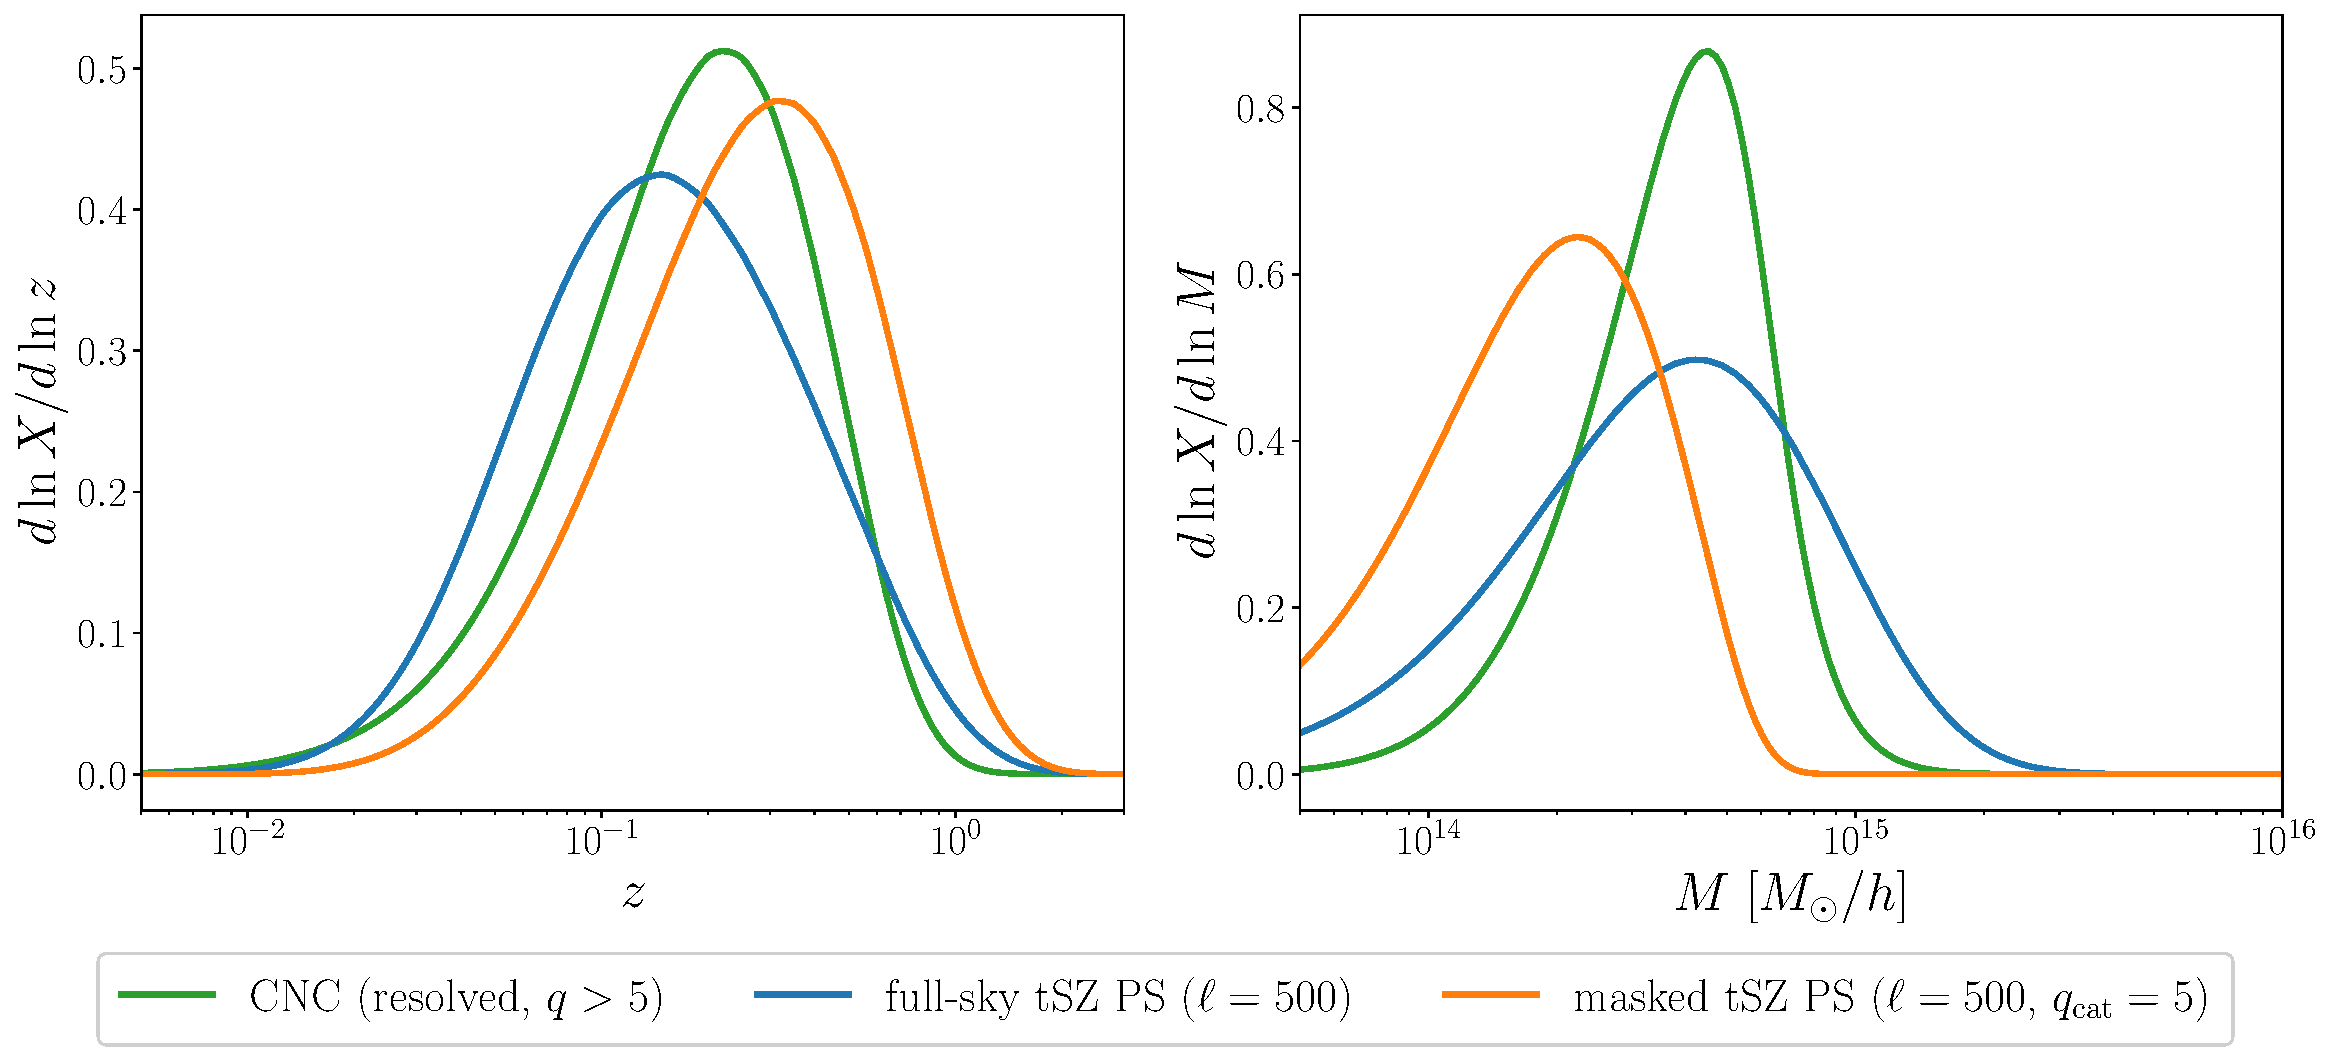
\includegraphics[width=\linewidth]{kernels_all_observables.pdf}
    \caption{\label{fig:kernels}%
    Redshift (top) and mass (bottom) kernels of the three observables at $\ell = 500$: the full-sky tSZ power spectrum, the masked tSZ power spectrum ($q_{\mathrm{cat}} = 5$), and the cluster number counts ($q > 5$).
    Masking shifts the power spectrum kernel from a mean mass of $\sim 6 \times 10^{14}\, M_\odot/h$ down to $\sim 3 \times 10^{14}\, M_\odot/h$ and to slightly higher redshift, while the counts remain sharply localised at the high-mass end.
    The split populations overlap only weakly, which is what makes the joint likelihood of Eq.~\eqref{eq:joint} self-consistent.}
\end{figure}

Figure~\ref{fig:kernels} illustrates the population split in terms of the mass and redshift kernels of the three observables: masking does not merely re-normalise the spectrum, it moves its support to genuinely lower masses, away from the counts.

%==============================================================================
\section{Validation on synthetic Planck-like skies}
\label{sec:synthetic}
%==============================================================================

\subsection{Halo-painting pipeline}
\label{sec:painting}

We generated synthetic data consistent with the likelihood forward model:
(i) haloes were Poisson-sampled from the halo mass function at the fiducial cosmology;
(ii) each halo received an intrinsic scatter factor per Eq.~\eqref{eq:scatter} with $\sigma_{\ln Y} = 0.173$;
(iii) GNFW profiles were painted at the scattered amplitudes onto full-sky HEALPix maps \citep{Gorski2005};
(iv) observed significances were drawn per Eq.~\eqref{eq:snr_mean} with a \textit{Planck}-like matched-filter noise curve;
(v) clusters with $q_{\mathrm{obs}} > q_{\mathrm{cat}} = 5$ were placed in the CNC catalogue and masked from the map; and
(vi) full-sky and masked bandpowers were measured on $18$ logarithmic bins.
For the foreground-contaminated case, the fixed templates of Eq.~\eqref{eq:fg_model} were added to the painted maps.
One thousand independent realisations were produced to characterise the bandpower distribution; single realisations were used as data vectors for the MCMC analyses.
The counts were binned into $n_z = 10$ redshift bins over $0.005 \le z \le 1$ and $n_q = 5$ geometric significance bins over $5 \le q \le 40$.

\subsection{Masking Gaussianises the bandpower distribution}
\label{sec:gaussianity}

\begin{figure}[t]
    \centering
    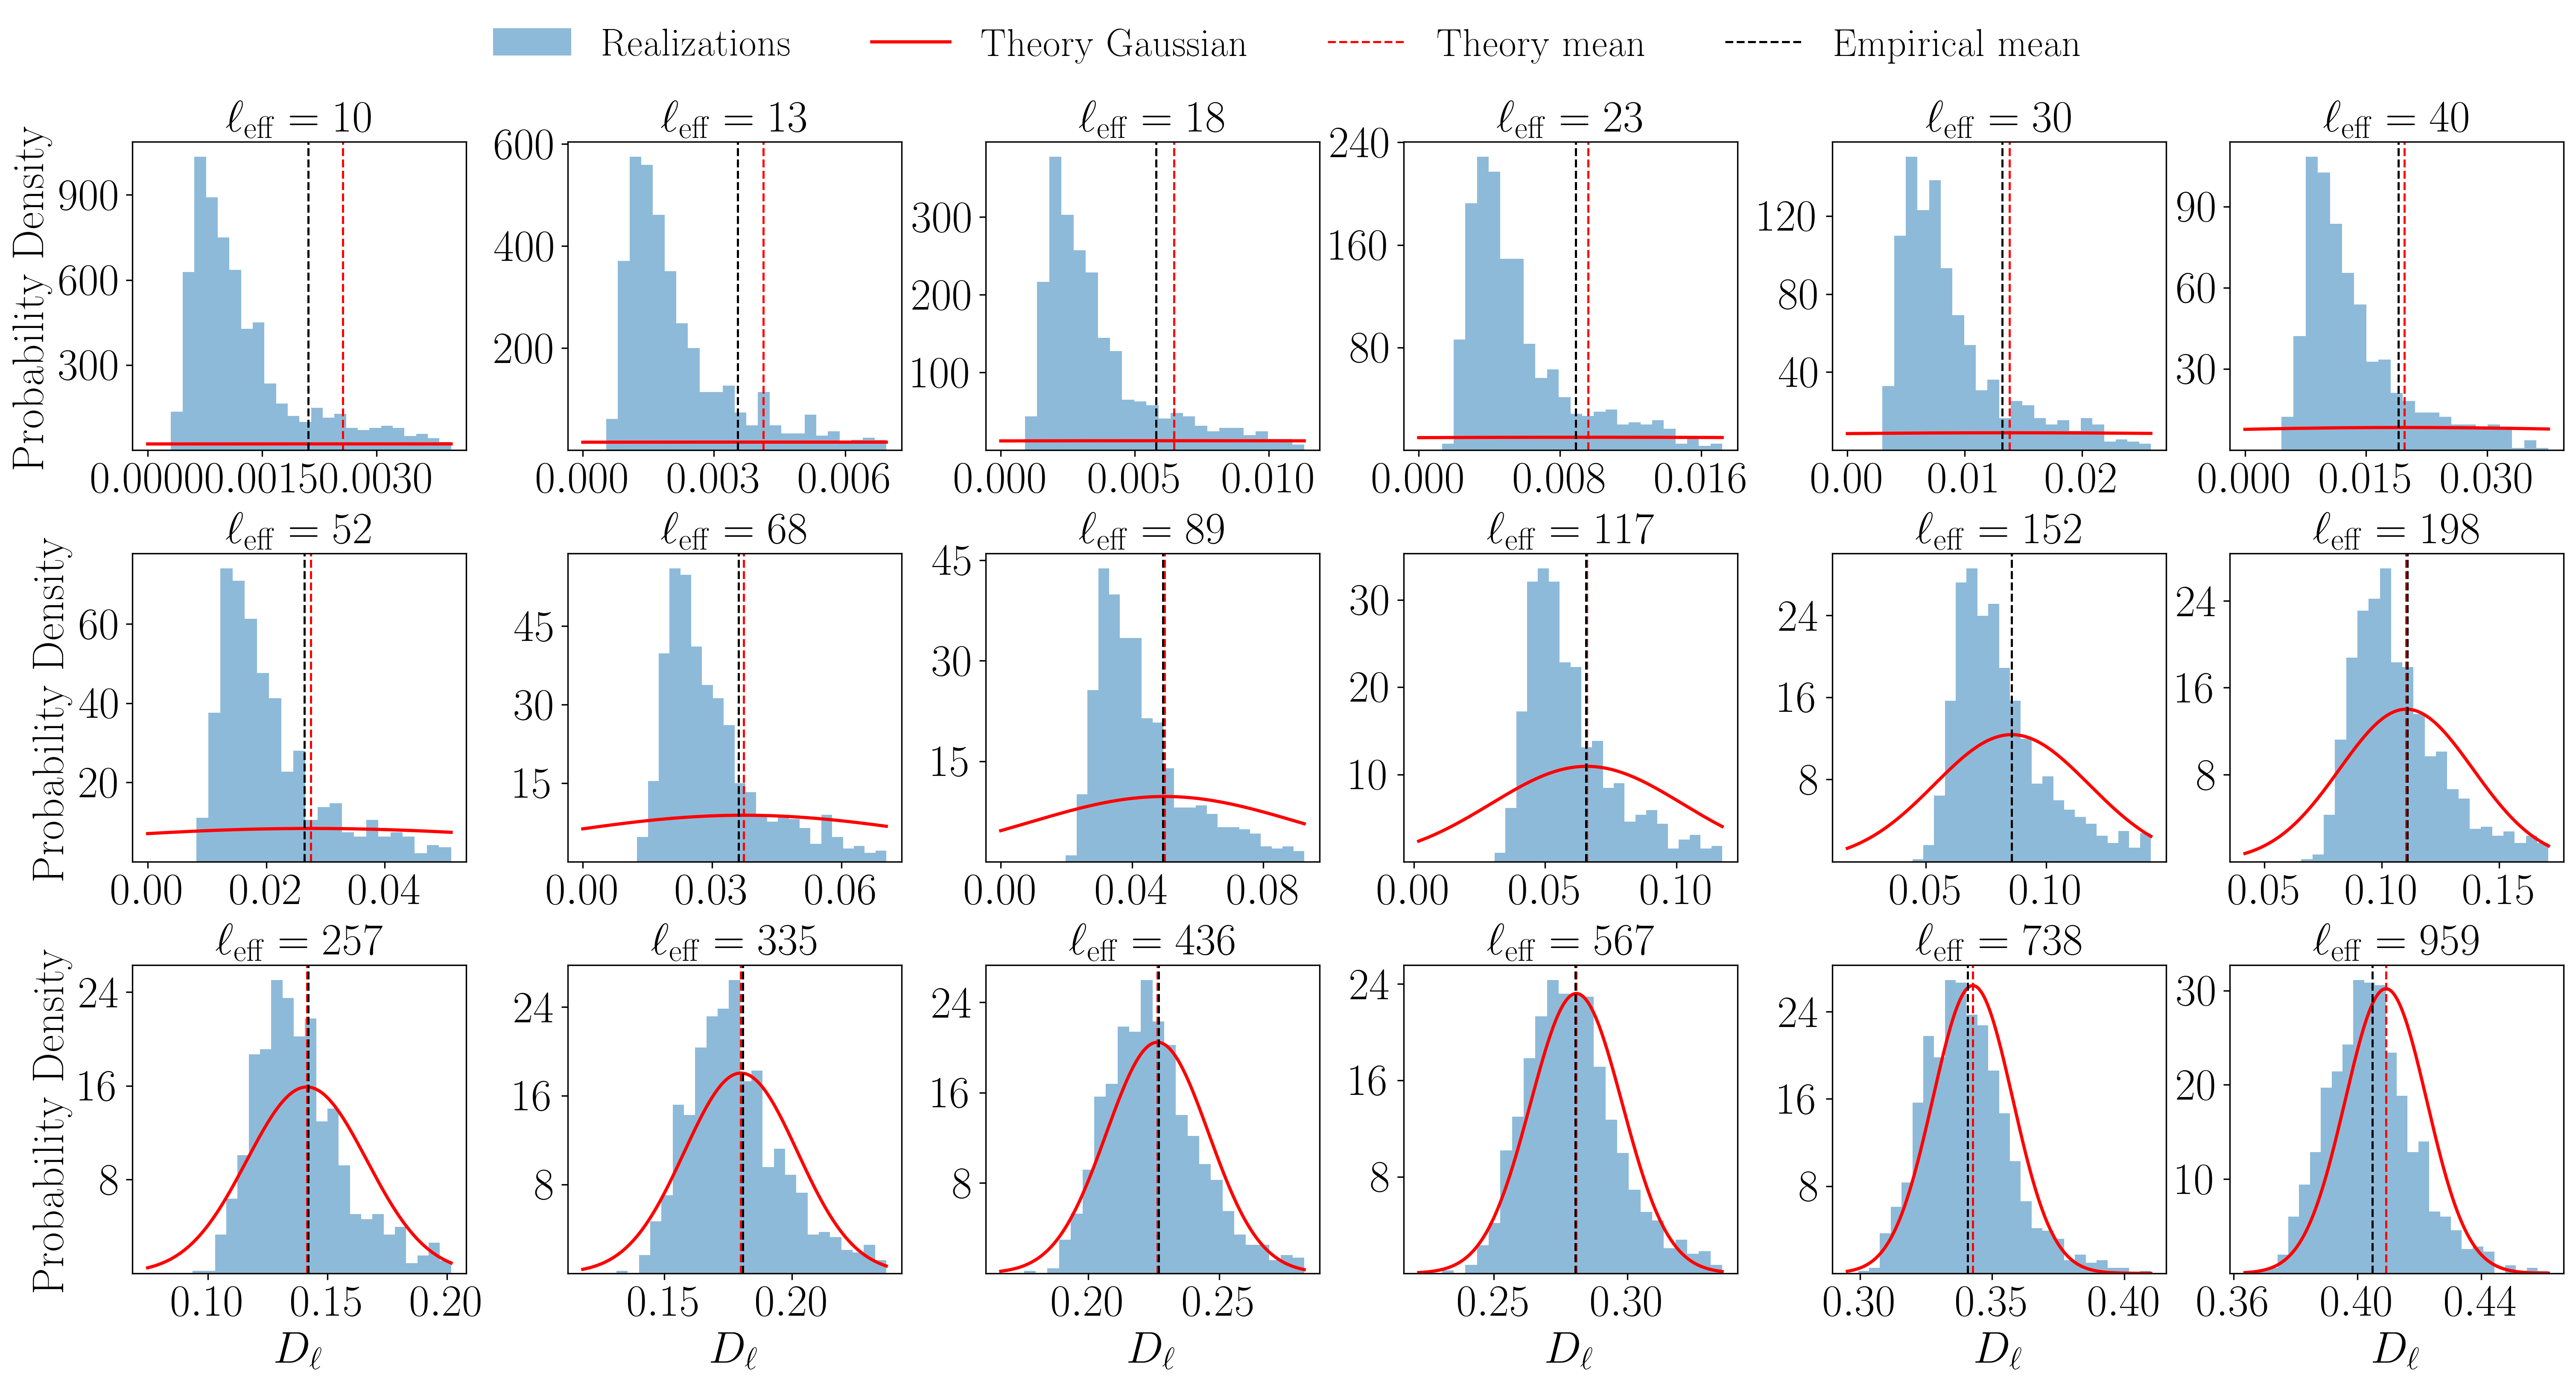
\includegraphics[width=\linewidth]{ps_scatter_fullsky.png}
    \caption{\label{fig:scatter_fullsky}%
    Full-sky binned bandpowers $D_\ell$ from $1000$ painted realisations (histograms) against the Gaussian prediction with the analytic covariance of Eq.~\eqref{eq:covariance} without masking (solid curves); vertical lines mark the theory (dashed) and empirical (dotted) means.
    At $\ell_{\mathrm{eff}} \lesssim 100$ the distributions are strongly right-skewed: single massive clusters shift entire realisations, and the Gaussian likelihood underpredicts the high-$D_\ell$ tail.}
\end{figure}

\begin{figure}[t]
    \centering
    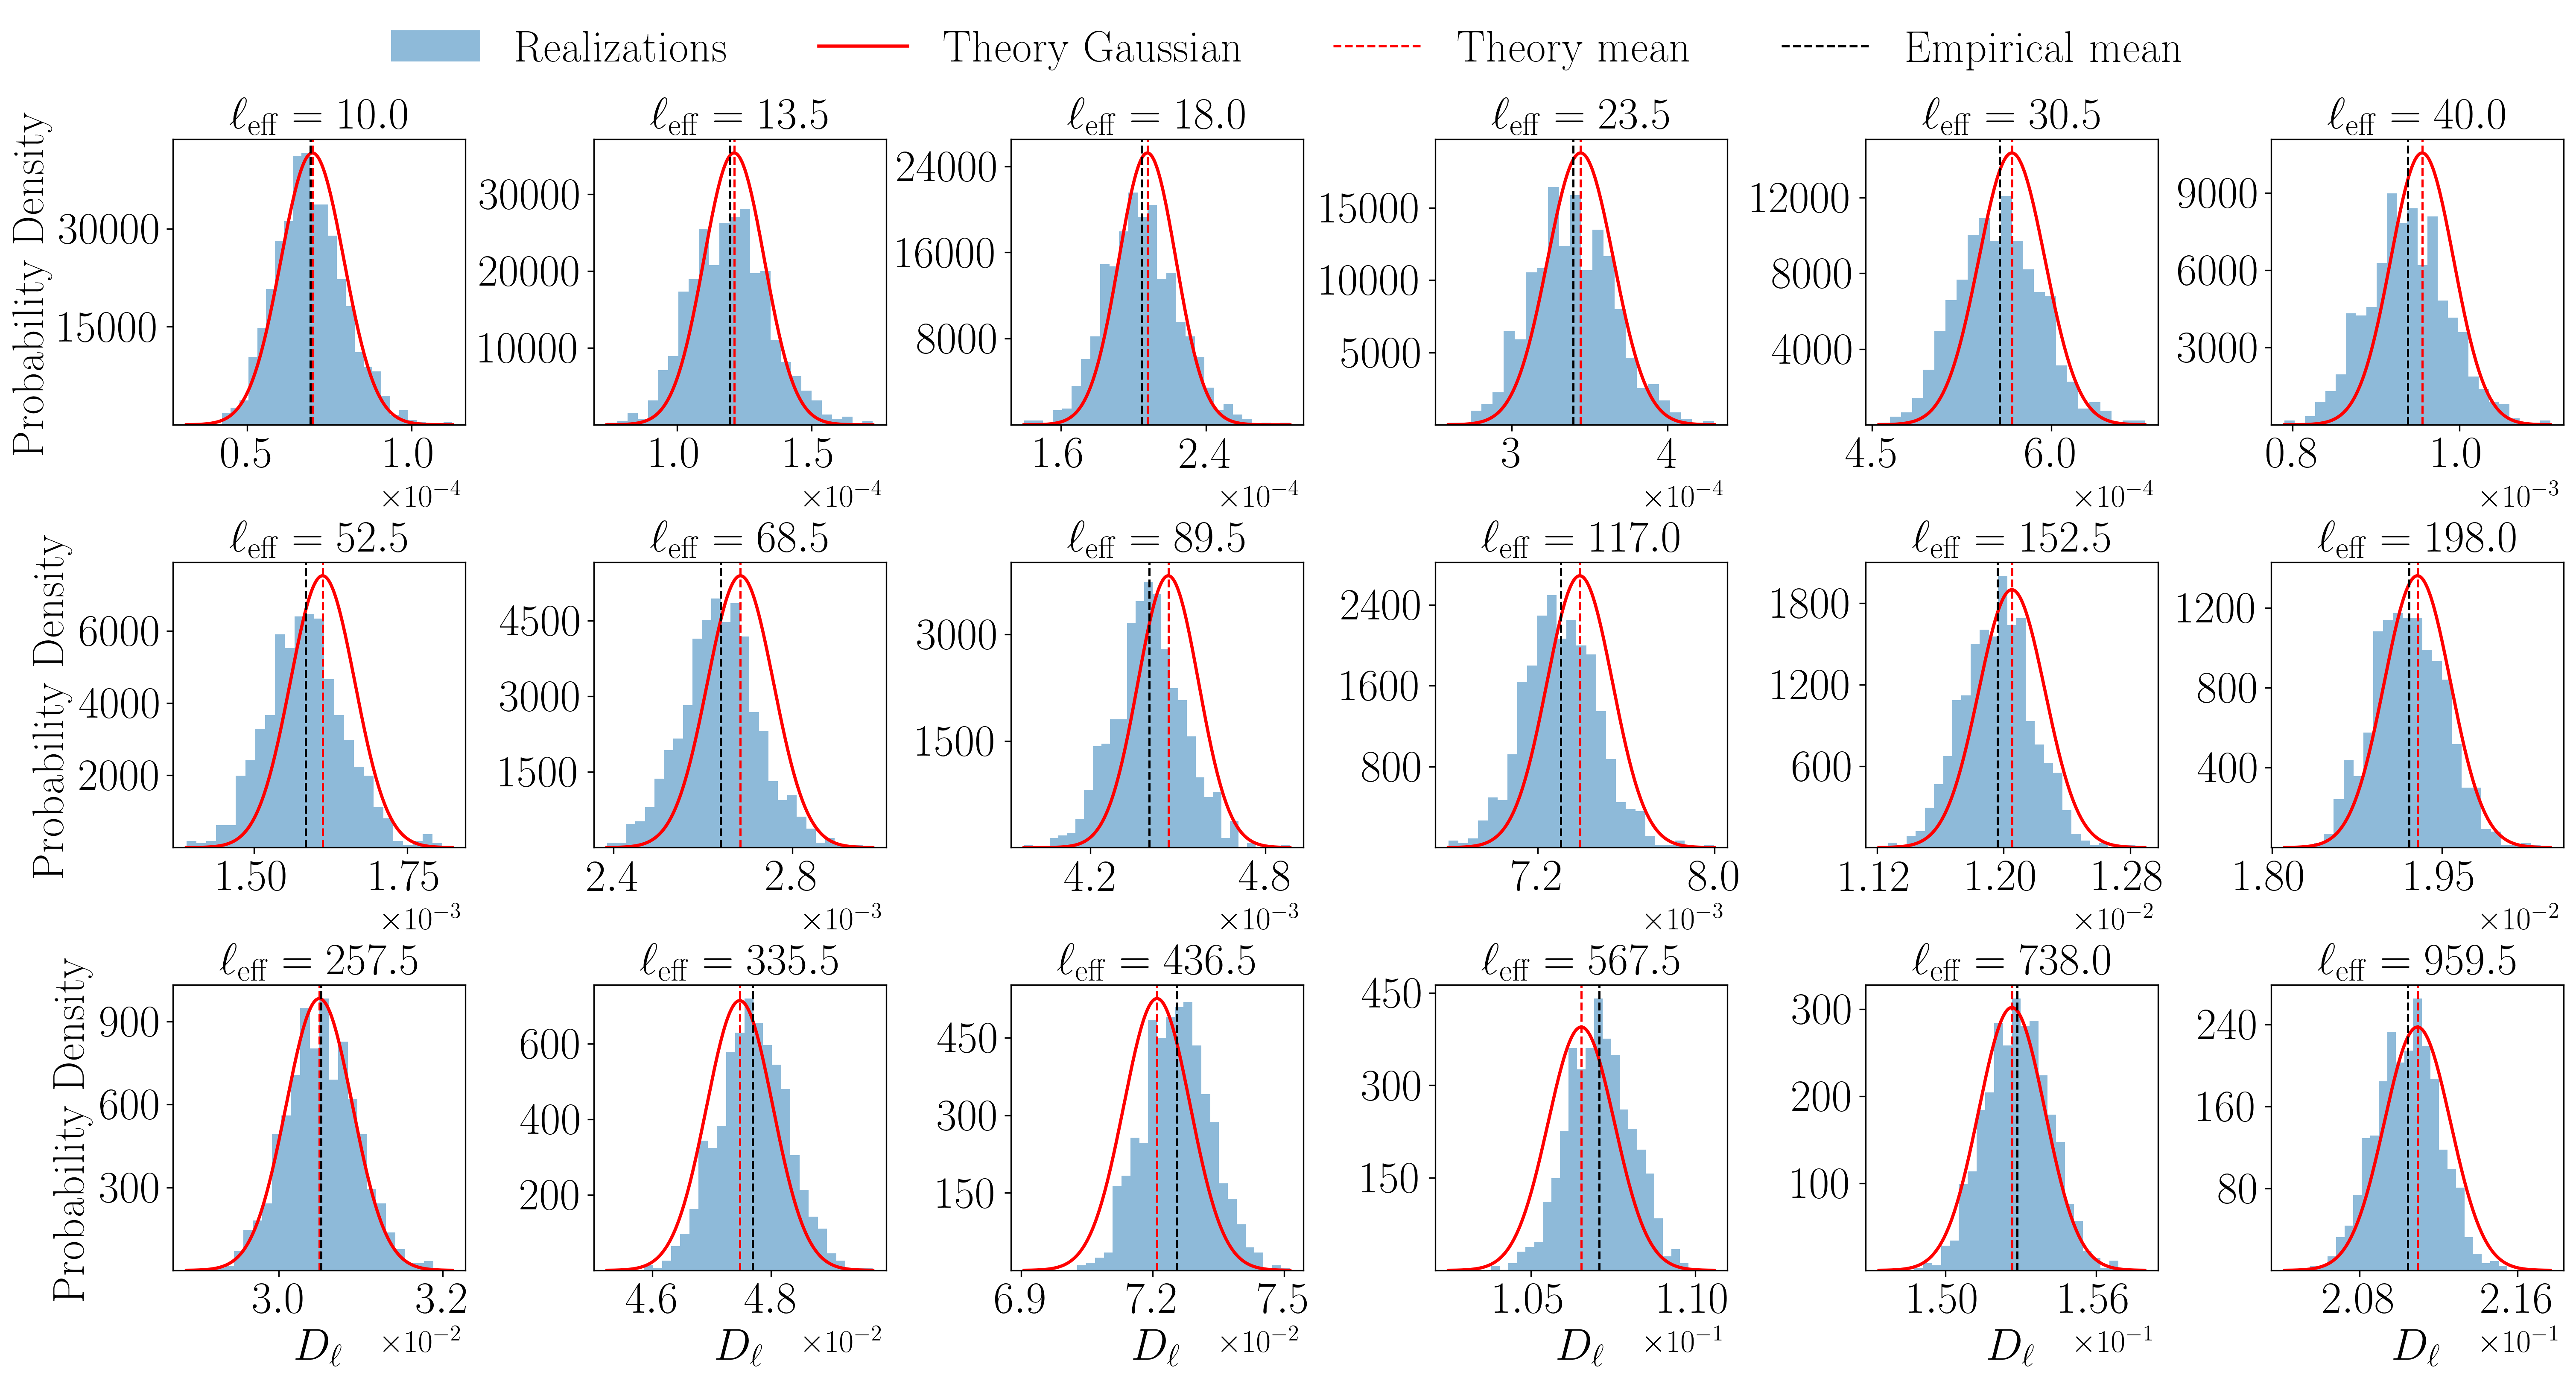
\includegraphics[width=\linewidth]{ps_scatter_masked.png}
    \caption{\label{fig:scatter_masked}%
    Same as Fig.~\ref{fig:scatter_fullsky} but for the masked spectra ($q_{\mathrm{cat}} = 5$), with the conditional-moment covariance of Eqs.~\eqref{eq:masked_trispec} and \eqref{eq:covariance}.
    Every bin is statistically consistent with the Gaussian prediction, including the lowest multipoles, and the empirical means agree with the $\mathcal{W}_2$-weighted theory of Eq.~\eqref{eq:masked_ps} at the $\sim 1\sigma$ level.}
\end{figure}

Figures~\ref{fig:scatter_fullsky} and \ref{fig:scatter_masked} contain the central statistical result of the synthetic stage.
Without masking, the bandpower distributions at $\ell_{\mathrm{eff}} \lesssim 100$ are visibly right-skewed, a well-known consequence of the Poisson rarity of the most massive haloes \citep{Zhang:2007psa,Horowitz:2017dsh,Rotti:2020rdl}; a Gaussian likelihood is then formally invalid exactly where the tSZ spectrum carries most of its cosmological weight.
After masking at $q_{\mathrm{cat}} = 5$, every one of the $18$ bins is statistically Gaussian, and both the mean and the variance agree with the conditional-moment theory: generalised-least-squares fits over $100$ foreground-contaminated realisations recover empirical-to-Fisher error ratios of $0.94$ for the masked spectra, compared with $0.82$ for the full-sky case.

\subsection{Joint constraints: signal-only case}
\label{sec:results_syn_nofg}

\begin{figure}[t]
    \centering
    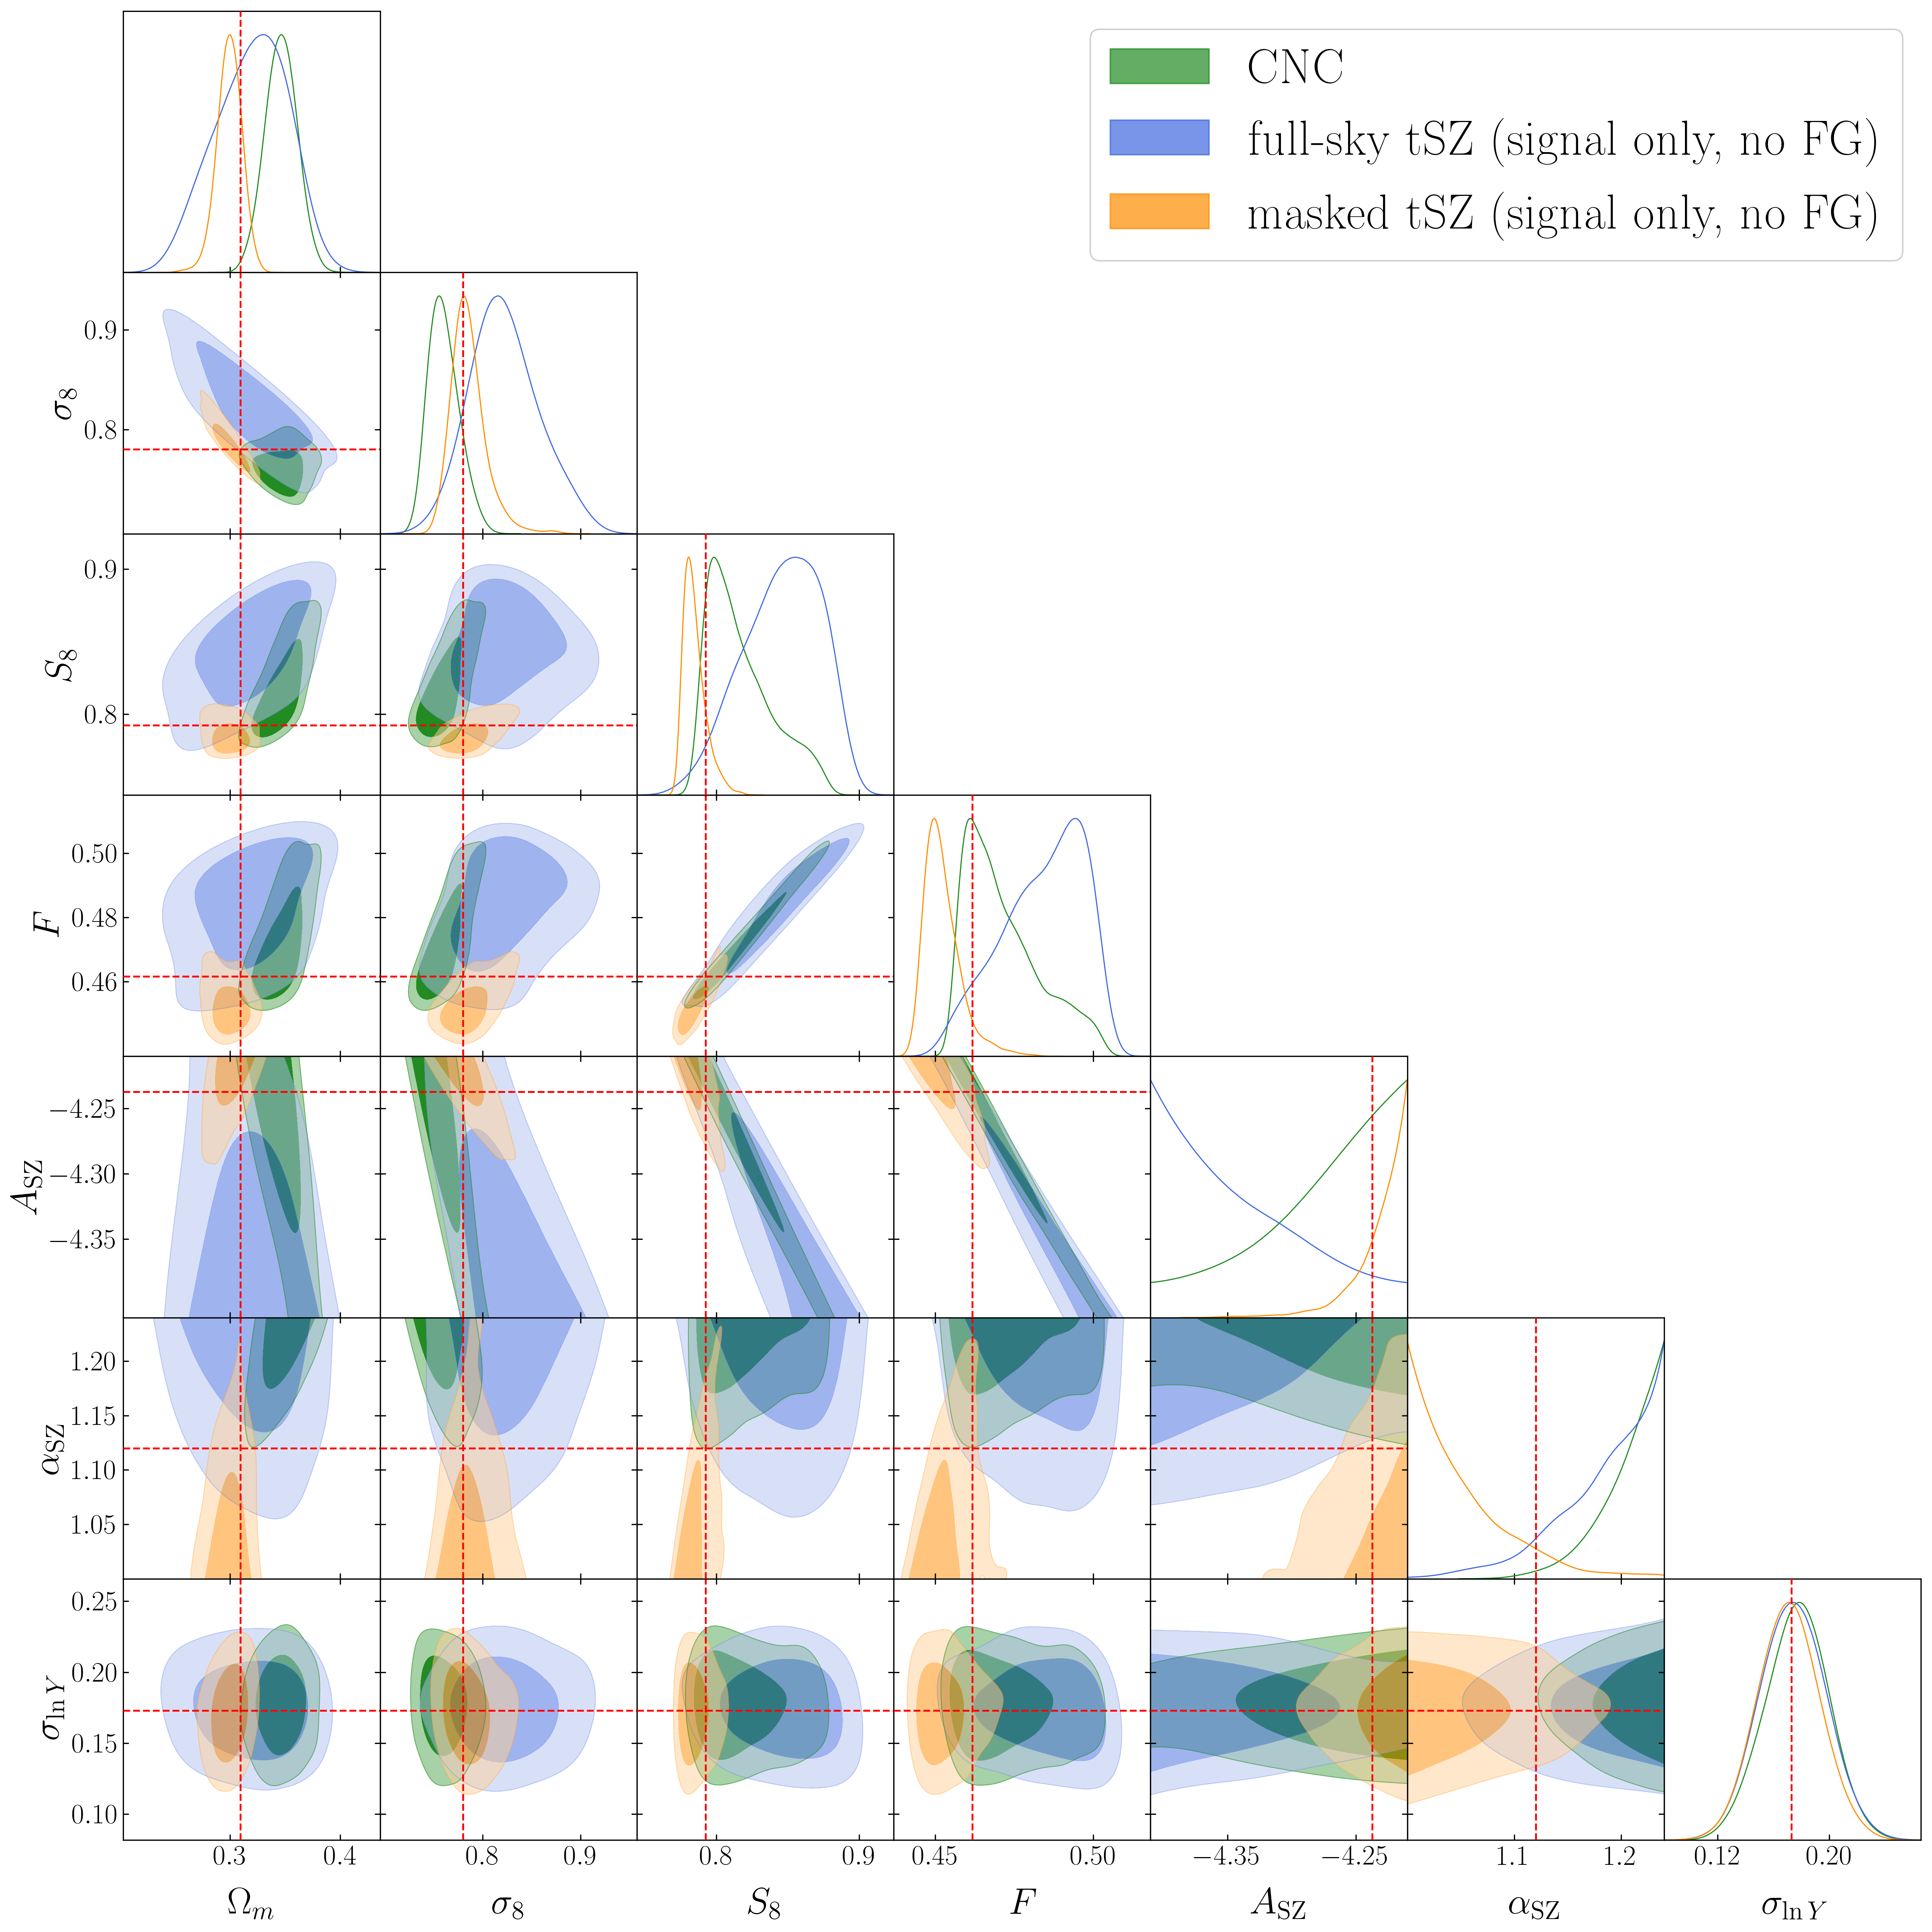
\includegraphics[width=0.95\linewidth]{triangle_signal_only_3contours.png}
    \caption{\label{fig:syn_single}%
    Posterior constraints ($68\%$ and $95\%$ credible regions) from the three single probes on the synthetic signal-only sky: CNC, full-sky tSZ power spectrum, and masked tSZ power spectrum ($q_{\mathrm{cat}} = 5$).
    Dashed lines mark the fiducial values.
    The full-sky spectrum constrains essentially the one-dimensional combination $F$ of Eq.~\eqref{eq:F_def}; the CNC posterior is offset high in $\Omega_{\mathrm{m}}$ by $+2.4\sigma$ (see text).}
\end{figure}

\begin{figure}[t]
    \centering
    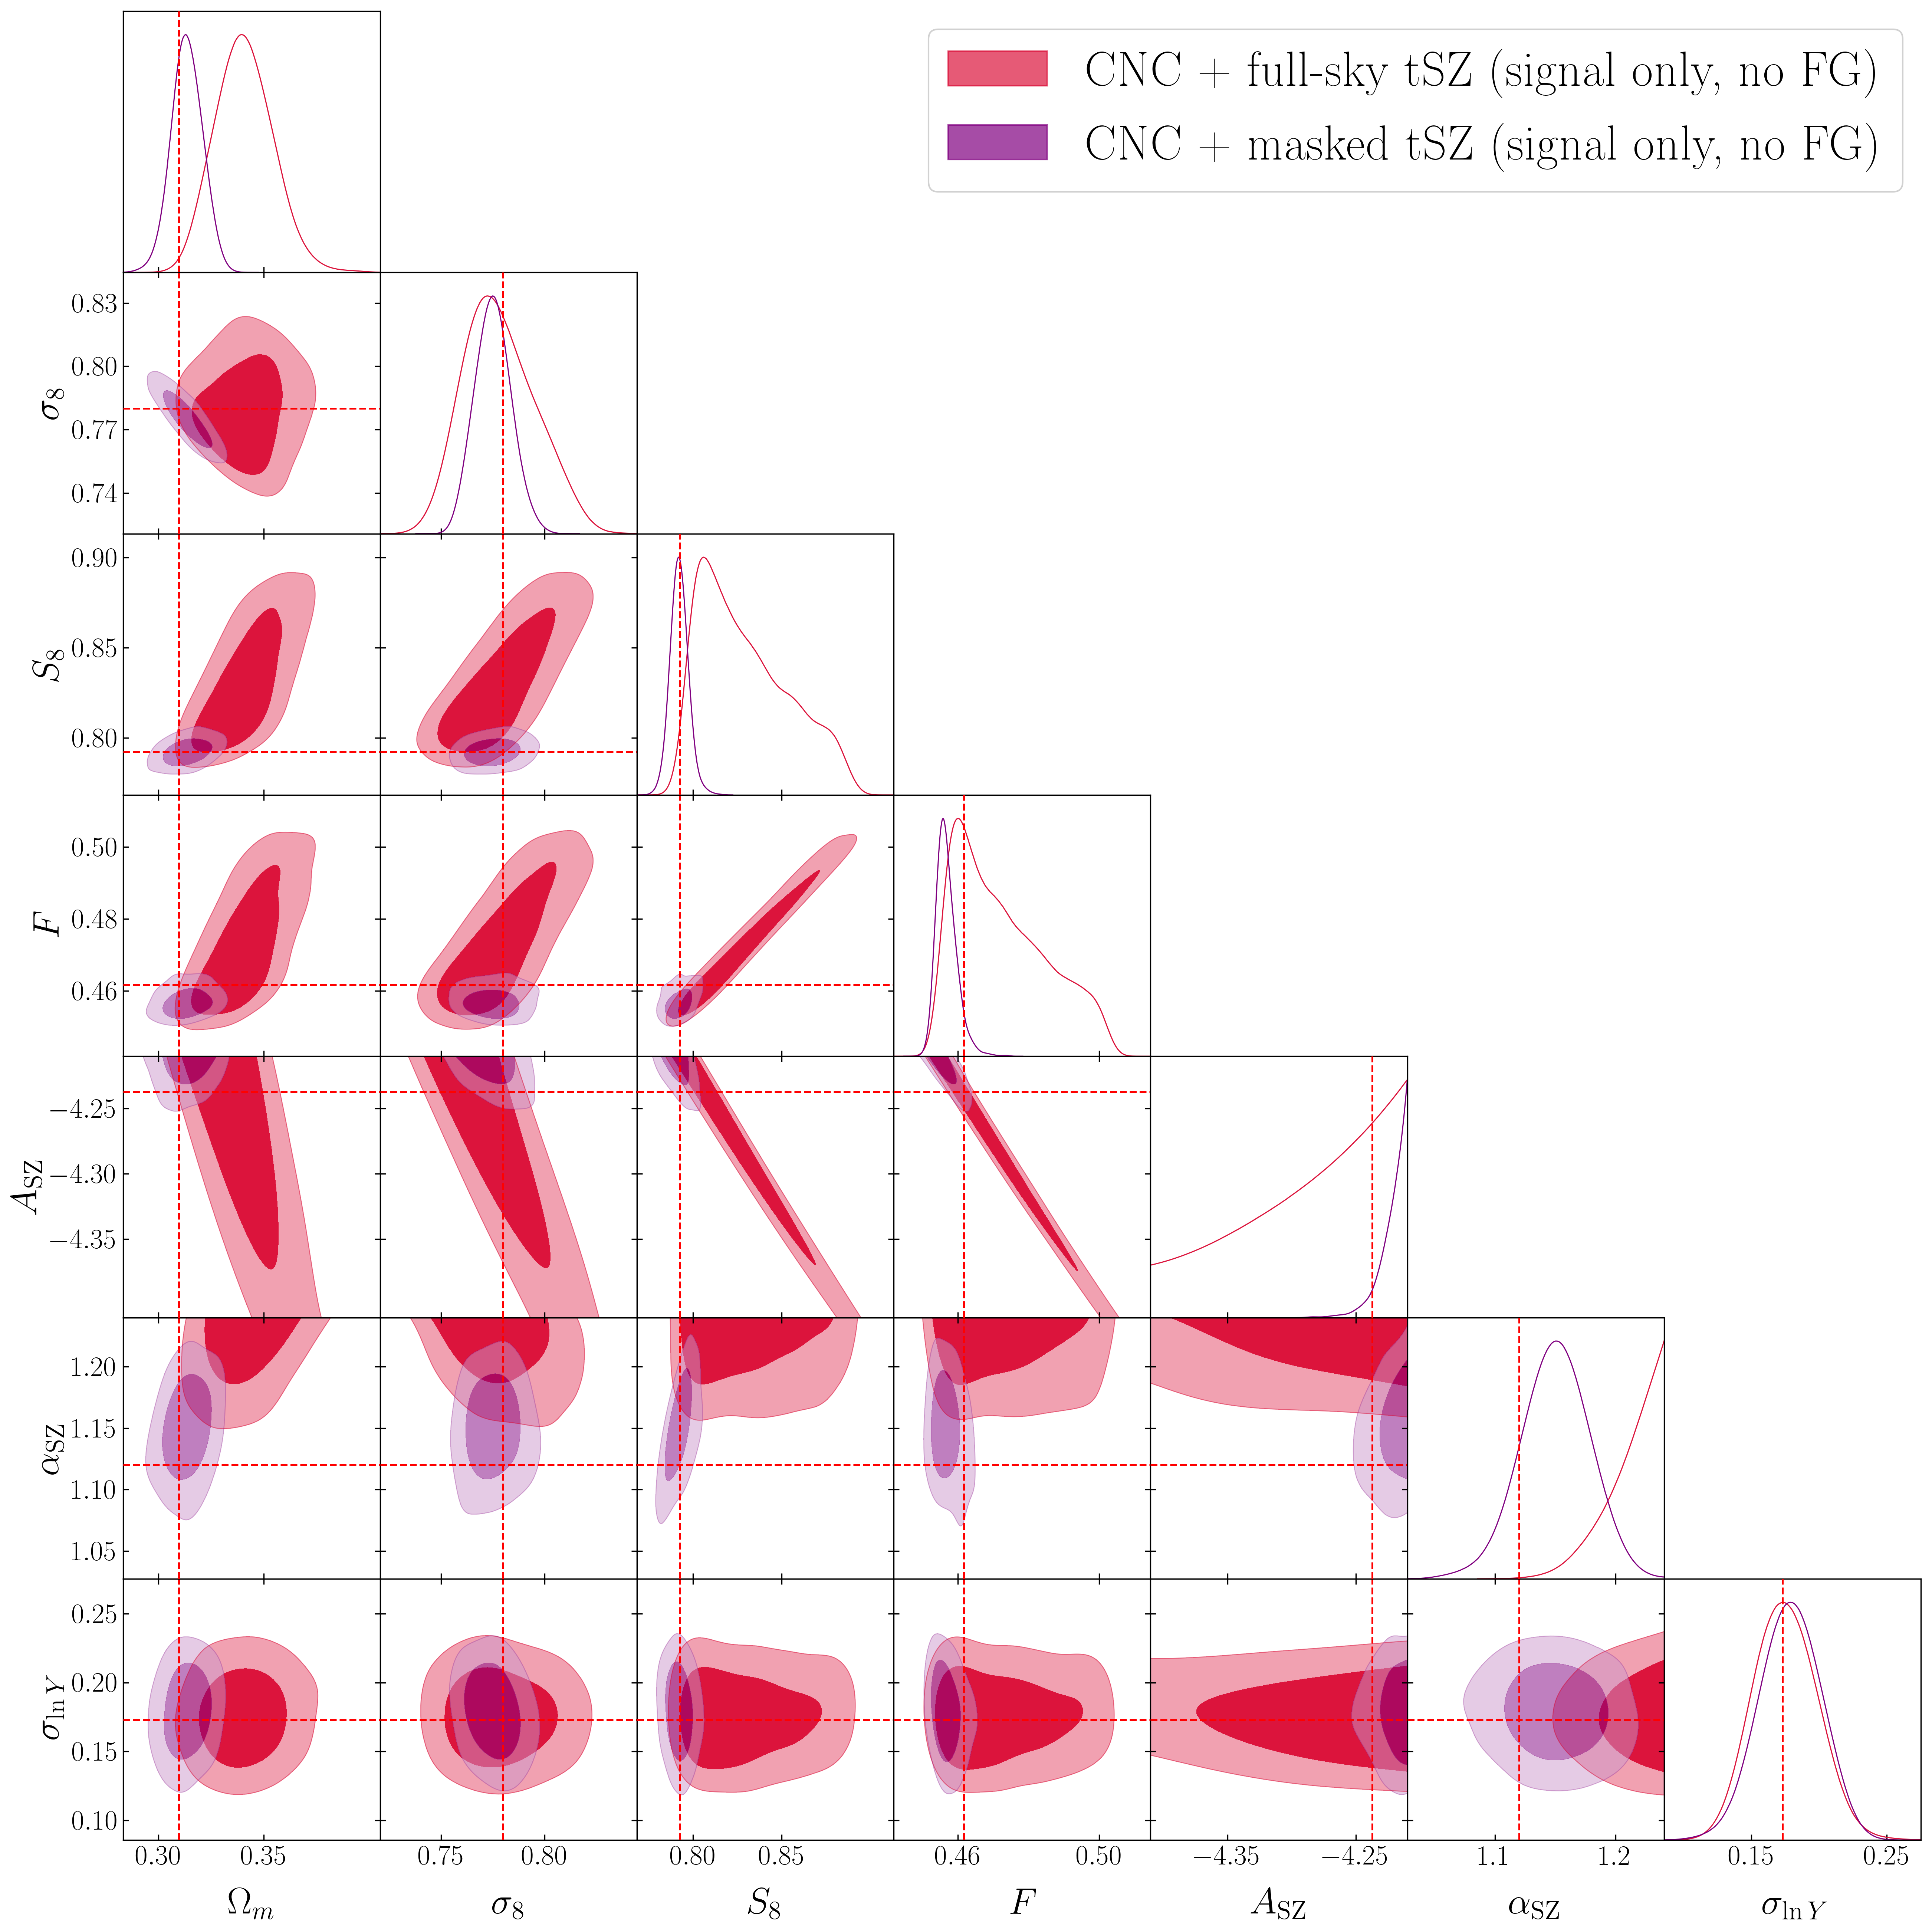
\includegraphics[width=0.95\linewidth]{triangle_signal_only_combined.png}
    \caption{\label{fig:syn_joint}%
    Joint posteriors on the synthetic signal-only sky: CNC plus full-sky tSZ versus CNC plus masked tSZ.
    The masked combination is the tightest on every parameter and pulls the CNC-induced $\Omega_{\mathrm{m}}$ offset back to $+0.5\sigma$.}
\end{figure}

Figures~\ref{fig:syn_single} and \ref{fig:syn_joint} compare the single-probe and joint posteriors in the signal-only case; Table~\ref{tab:constraints} lists the marginalised constraints.
The joint CNC plus masked-tSZ chain reaches $\Omega_{\mathrm{m}} = 0.314 \pm 0.008$, $\sigma_8 = 0.775 \pm 0.009$, and $F = 0.457 \pm 0.003$, factors of $1.4$ to $5$ tighter than any single probe (a factor $4$ on $F$ relative to the counts alone).
The combination with the \emph{full-sky} spectrum is weaker on every parameter and inherits the counts' $\Omega_{\mathrm{m}}$ offset almost unchanged ($+2.2\sigma$), because the low-$\ell$ non-Gaussian scatter deprives the full-sky spectrum of the weight needed to pull the solution back; masking restores that weight.
The CNC offset itself ($\Omega_{\mathrm{m}}$ high by $+2.4\sigma$, $\sigma_8$ low by $-1.2\sigma$ in this realisation) traces to the interaction of the fixed hydrostatic bias with the sample scatter, and is the prototype of the bias-variance trade-off discussed next.

\begin{table*}
\caption{\label{tab:constraints}%
Marginalised constraints ($68\%$) on the synthetic skies.
$S_8 \equiv \sigma_8 (\Omega_{\mathrm{m}}/0.3)^{1/2}$; $F$ is defined in Eq.~\eqref{eq:F_def}.
Fiducial values are $\Omega_{\mathrm{m}} = 0.31$, $\sigma_8 = 0.78$.}
\begin{ruledtabular}
\begin{tabular}{lcccc}
Data combination & $\Omega_{\mathrm{m}}$ & $\sigma_8$ & $S_8$ & $F$ \\
\hline
\multicolumn{5}{l}{\emph{Signal only}}\\
CNC & $0.346 \pm 0.015$ & $0.760 \pm 0.016$ & $0.817 \pm 0.023$ & $0.471 \pm 0.012$ \\
Full-sky tSZ & $0.320 \pm 0.033$ & $0.822 \pm 0.037$ & $0.846 \pm 0.028$ & $0.484 \pm 0.013$ \\
Masked tSZ & $0.300 \pm 0.012$ & $0.786 \pm 0.019$ & $0.785 \pm 0.008$ & $0.452 \pm 0.006$ \\
CNC + full-sky tSZ & $0.341 \pm 0.014$ & $0.778 \pm 0.018$ & $0.829 \pm 0.026$ & $0.472 \pm 0.013$ \\
CNC + masked tSZ & $0.314 \pm 0.008$ & $0.775 \pm 0.009$ & $0.792 \pm 0.005$ & $0.457 \pm 0.003$ \\
\hline
\multicolumn{5}{l}{\emph{Signal plus foregrounds}}\\
Full-sky tSZ & $0.325 \pm 0.041$ & $0.830 \pm 0.047$ & $0.859 \pm 0.035$ & $0.499 \pm 0.018$ \\
Masked tSZ & $0.307 \pm 0.036$ & $0.792 \pm 0.056$ & $0.798 \pm 0.040$ & $0.466 \pm 0.023$ \\
CNC + full-sky tSZ & $0.352 \pm 0.015$ & $0.764 \pm 0.017$ & $0.827 \pm 0.025$ & $0.477 \pm 0.013$ \\
CNC + masked tSZ & $0.342 \pm 0.014$ & $0.758 \pm 0.015$ & $0.810 \pm 0.019$ & $0.468 \pm 0.010$ \\
\end{tabular}
\end{ruledtabular}
\end{table*}

\subsection{Foreground residuals limit the joint analysis}
\label{sec:results_syn_fg}

\begin{figure}[t]
    \centering
    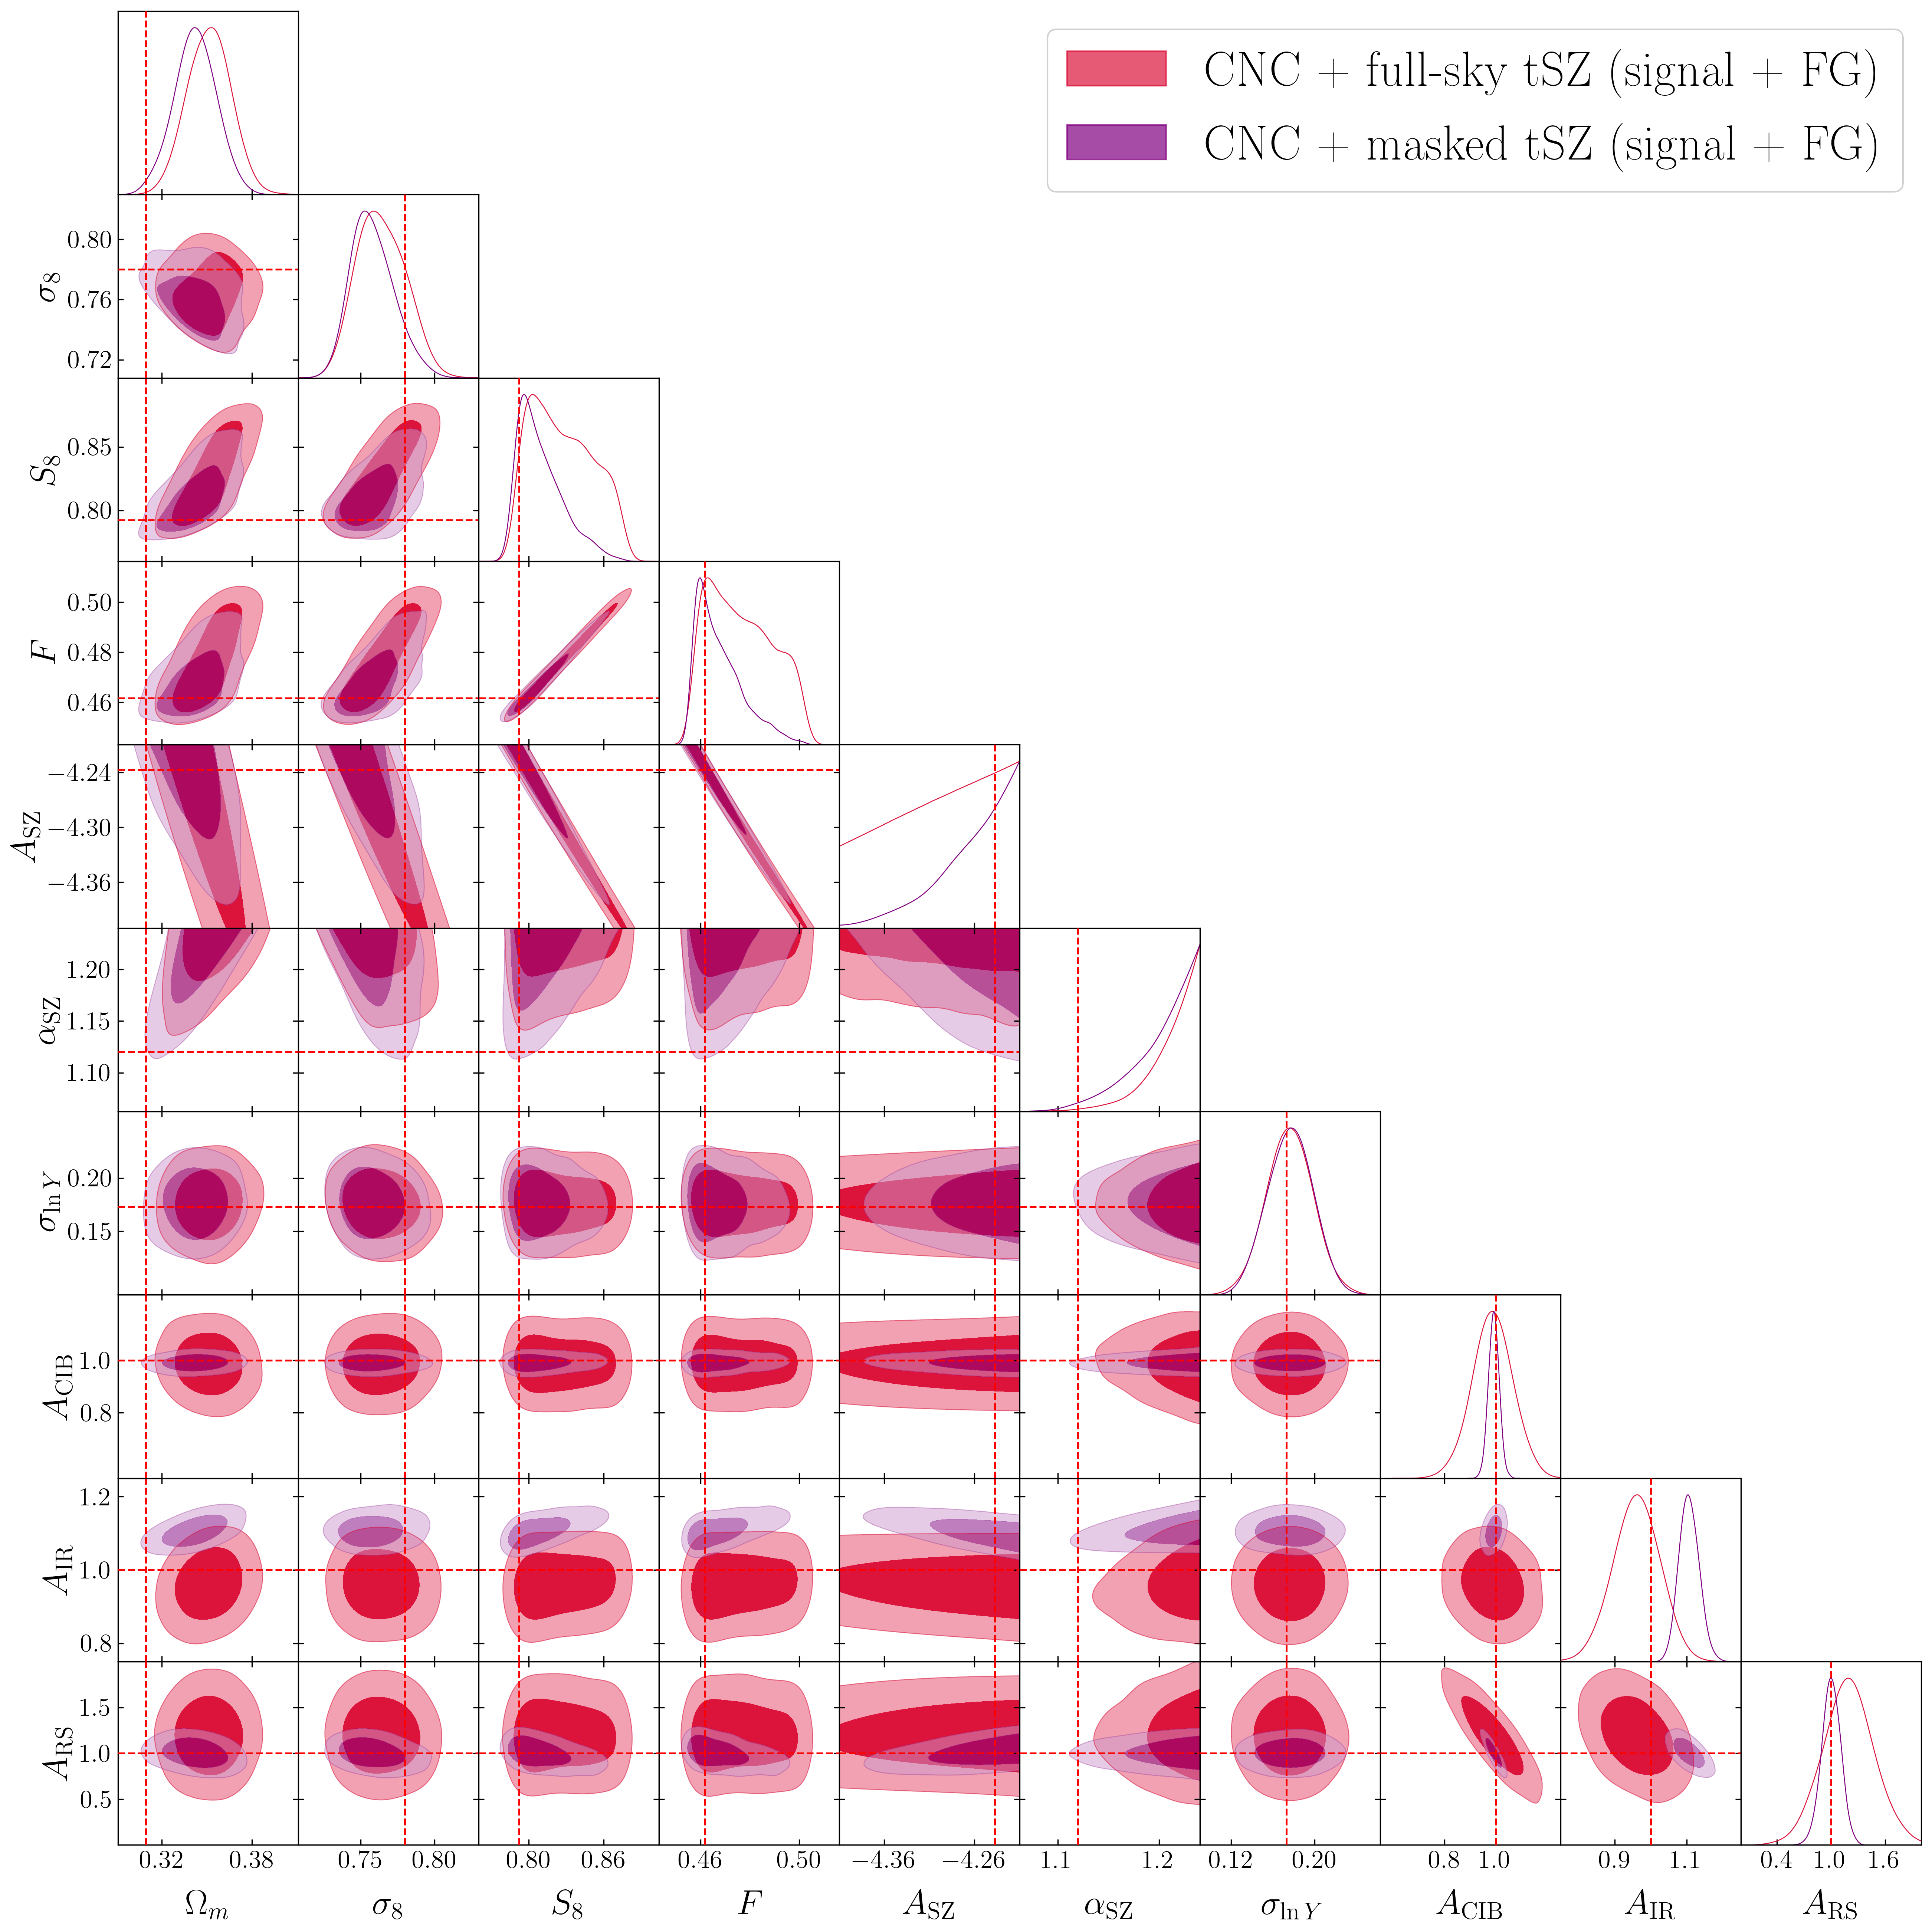
\includegraphics[width=0.95\linewidth]{triangle_signal_plus_fg_combined.png}
    \caption{\label{fig:syn_fg}%
    Joint posteriors on the foreground-contaminated synthetic sky, marginalising over the three free template amplitudes of Eq.~\eqref{eq:fg_model} with $\mathcal{N}(1, 0.5)$ priors.
    The joint gains persist, but the CNC-induced $\Omega_{\mathrm{m}}$ offset now propagates into the combination and is absorbed by the most tSZ-degenerate template amplitude, $A_{\mathrm{IR}}$, which is biased by $+3.8\sigma$.}
\end{figure}

With the foreground templates added to the maps and their amplitudes marginalised, the single-probe errors on $\Omega_{\mathrm{m}}$ roughly double, and the joint CNC plus masked-tSZ chain still improves on the masked spectrum alone by factors of $2.6$, $3.7$, and $2.3$ on $\sigma(\Omega_{\mathrm{m}})$, $\sigma(\sigma_8)$, and $\sigma(F)$ respectively (Fig.~\ref{fig:syn_fg} and Table~\ref{tab:constraints}).
The limitation is no longer statistical.
A Fisher scan over masking thresholds shows that masking rotates and contracts the degeneracy between the tSZ amplitude and each template by more than an order of magnitude as $q_{\mathrm{cat}}$ decreases, but the infrared-source template retains the $\ell$ dependence closest to the masked tSZ shape and stays degenerate.
In the joint chain this template absorbs the residual tension between the counts (which prefer high $\Omega_{\mathrm{m}}$) and the masked spectrum: $A_{\mathrm{IR}} = 1.106 \pm 0.028$, a $+3.8\sigma$ bias, while $A_{\mathrm{CIB}} = 0.991 \pm 0.021$ and $A_{\mathrm{RS}} = 1.002 \pm 0.108$ remain unbiased.
The joint analysis is therefore \emph{limited by the modelling of the foreground residuals}: with a fixed, incomplete template basis, parameter shifts leak preferentially into whichever component is most degenerate with the unresolved tSZ shape.
An external prior on $B$, or a physically parametrised CIB and IR model, would break this leakage.

%==============================================================================
\section{Application to the FLAMINGO simulations}
\label{sec:flamingo}
%==============================================================================

The synthetic stage establishes that the estimator works when the data are generated by the model.
We now drop that safety net and apply the same masking machinery to the FLAMINGO hydrodynamical simulations, in which the pressure content of haloes emerges from calibrated subgrid physics rather than from a GNFW profile.
The goals are the three questions listed in the Introduction: the multipole dependence of progressive masking, the decorrelation of the two probes, and the effect of masking on feedback sensitivity.
We do not perform parameter inference on FLAMINGO in this paper; a single simulated sky constrains a joint fit only weakly, and the known offset between the Tinker08 mass function and the FLAMINGO halo abundance would dominate the error budget (see Sec.~\ref{sec:discussion}).

\subsection{Simulations, maps, and catalogues}
\label{sec:flamingo_data}

FLAMINGO \citep{Schaye2023,Kugel2023} is a suite of cosmological hydrodynamical simulations run at the D3A cosmology ($\Omega_{\mathrm{m}} = 0.306$, $\sigma_8 = 0.807$, $h = 0.681$, $n_s = 0.967$).
We used two elements of the suite:
\begin{itemize}
    \item \textbf{L2p8\_m9}: the $(2.8\,\mathrm{Gpc})^3$ flagship box, whose light-cone provides a full-sky Compton-$y$ map to $z = 3$ at HEALPix resolution $N_{\mathrm{side}} = 4096$, together with a SOAP halo catalogue restricted to $M_{500\mathrm{c}} > 5 \times 10^{13}\, M_\odot$ and $z < 3$ ($1\,555\,542$ objects) carrying the measured Compton parameters $Y_{500\mathrm{c}}$ of each halo.
    \item \textbf{L1\_m9}: the $(1\,\mathrm{Gpc})^3$ box at the same resolution, available for the fiducial calibration and eight astrophysical-feedback variants \citep{Kugel2023}: cluster gas fractions shifted by $\pm 2$, $-4$, and $-8$ times the calibration uncertainty ($\mathrm{fgas} \pm N\sigma$), a stellar-mass shift ($M_* - 1\sigma$), kinetic jet AGN feedback (Jet), and two combined variants.
    For each variant we built the light-cone Compton-$y$ map at $N_{\mathrm{side}} = 4096$ and the matched halo catalogue ($M_{500\mathrm{c}} > 5 \times 10^{13}\, M_\odot$, $z < 3$).
\end{itemize}
Detection significances were assigned to every halo through the forward model of Sec.~\ref{sec:snr}, with the matched-filter noise curve $\sigma_{\mathrm{noise}}(\theta_{500})$ of the \textit{Planck} SZiFi multi-frequency matched filter \citep{Zubeldia2024b}.
For L2p8\_m9 the significance uses the halo's measured $Y_{500\mathrm{c}}$ with the A10 shape at $B = 1$; for L1\_m9 the significance uses the parametric A10 amplitude with $B = 1.35$, the value at which the A10 prediction matches the FLAMINGO Compton signals of massive clusters, plus log-normal scatter with $\sigma_{\ln Y} = 0.173$.
Within each analysis the same convention defines both the mask and the catalogue, which is the only consistency the method requires.

The map-side pipeline is identical in all cases: a disc of radius $5\,\theta_{500}$ is masked around every cluster above threshold, the mask is apodised with a $0.5\deg$ C1 kernel, bandpowers are estimated with the mode-decoupling pseudo-$C_\ell$ estimator of \texttt{NaMaster} \citep{Alonso2019} in linear bins of width $\Delta\ell = 30$ to $\ell_{\mathrm{max}} = 6000$, and the HEALPix pixel window is deconvolved.

\subsection{Progressive SNR masking of the tSZ spectrum}
\label{sec:flamingo_snr}

\begin{figure}[t]
    \centering
    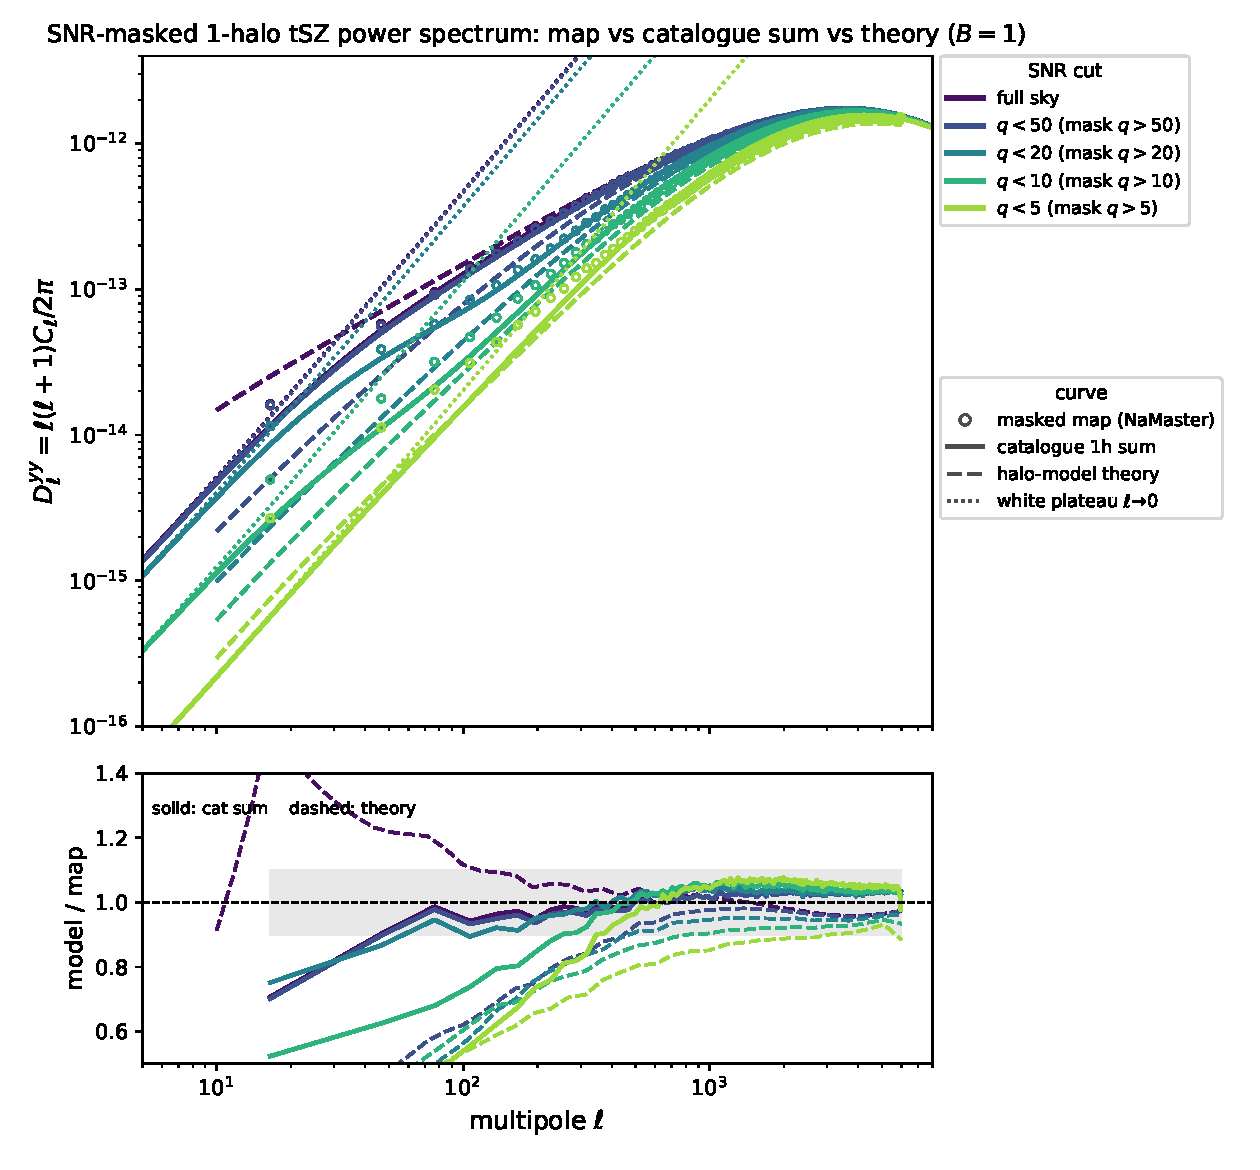
\includegraphics[width=\linewidth]{flamingo_snr_masked_ps.pdf}
    \caption{\label{fig:flamingo_snr}%
    L2p8\_m9 tSZ power spectrum under progressive SNR masking.
    Colours denote the threshold (full sky and $q_{\mathrm{cat}} = 50, 20, 10, 5$); within each colour, circles show the masked map bandpowers, solid lines the model-free catalogue summation of Eq.~\eqref{eq:cat_sum} over the surviving haloes, dashed lines the completeness-weighted halo-model theory, and dotted lines the white plateau $C_{\mathrm{white}} = \sum_{\mathrm{surv}} Y_{\mathrm{ang}}^2 / 4\pi$.
    The lower panel shows the ratio of each prediction to the map.
    The catalogue sum tracks the map to a median of $1.028$ over $400 < \ell < 6000$ (full sky); its low-$\ell$ deficit is the omitted two-halo term, which the halo-model theory (dashed) supplies.}
\end{figure}

For a catalogue with measured Compton parameters, the masked one-halo spectrum can be predicted without any mass function or pressure model, by direct summation over the surviving haloes:
\begin{equation}
    C_\ell^{\mathrm{1h,cat}}
    = \frac{1}{4\pi} \sum_{i \,\in\, \mathcal{S}_{\mathrm{PS}}}
    \bigl| Y_{\mathrm{ang},i}\, \hat G(\ell\, \theta_{500,i}) \bigr|^2,
    \label{eq:cat_sum}
\end{equation}
where $Y_{\mathrm{ang},i} = Y_i / d_A^2(z_i)$ is the angular integrated Compton parameter in steradians and $\hat G$ is the normalised Fourier transform of the fixed GNFW shape, with $\hat G \to 1$ as $\ell \to 0$.
In that limit Eq.~\eqref{eq:cat_sum} tends to the white plateau $C_{\mathrm{white}} = \sum Y_{\mathrm{ang}}^2/4\pi$, the shot-noise level set entirely by the brightest surviving objects.

Figure~\ref{fig:flamingo_snr} compares three independent estimates of the masked spectrum on L2p8\_m9: the masked map, the catalogue summation, and the completeness-weighted halo-model theory of Eq.~\eqref{eq:masked_ps}.
Three results stand out.
First, the catalogue sum reproduces the map bandpowers with a median ratio of $1.028$ over $400 < \ell < 6000$ on the full sky, confirming that the map power at these scales is the one-halo contribution of the catalogued haloes.
Second, masking removes power monotonically but extremely unevenly across thresholds: the white plateau falls by a factor of $23$ from the full sky ($C_{\mathrm{white}} = 2.9 \times 10^{-16}$) to $q_{\mathrm{cat}} = 5$ ($1.3 \times 10^{-17}$), even though the $q > 5$ clusters cost only $16$ per cent of the sky ($f_{\mathrm{sky}} = 0.84$).
Third, the halo-model theory brackets the masked map together with the catalogue sum at every threshold; at the strongest cuts the probabilistic completeness weighting removes slightly more power at high $\ell$ than the hard survivor cut, and the two predictions enclose the map.

\subsection{Isolating halo populations: mass and redshift masking}
\label{sec:flamingo_mz}

\begin{figure*}[t]
    \centering
    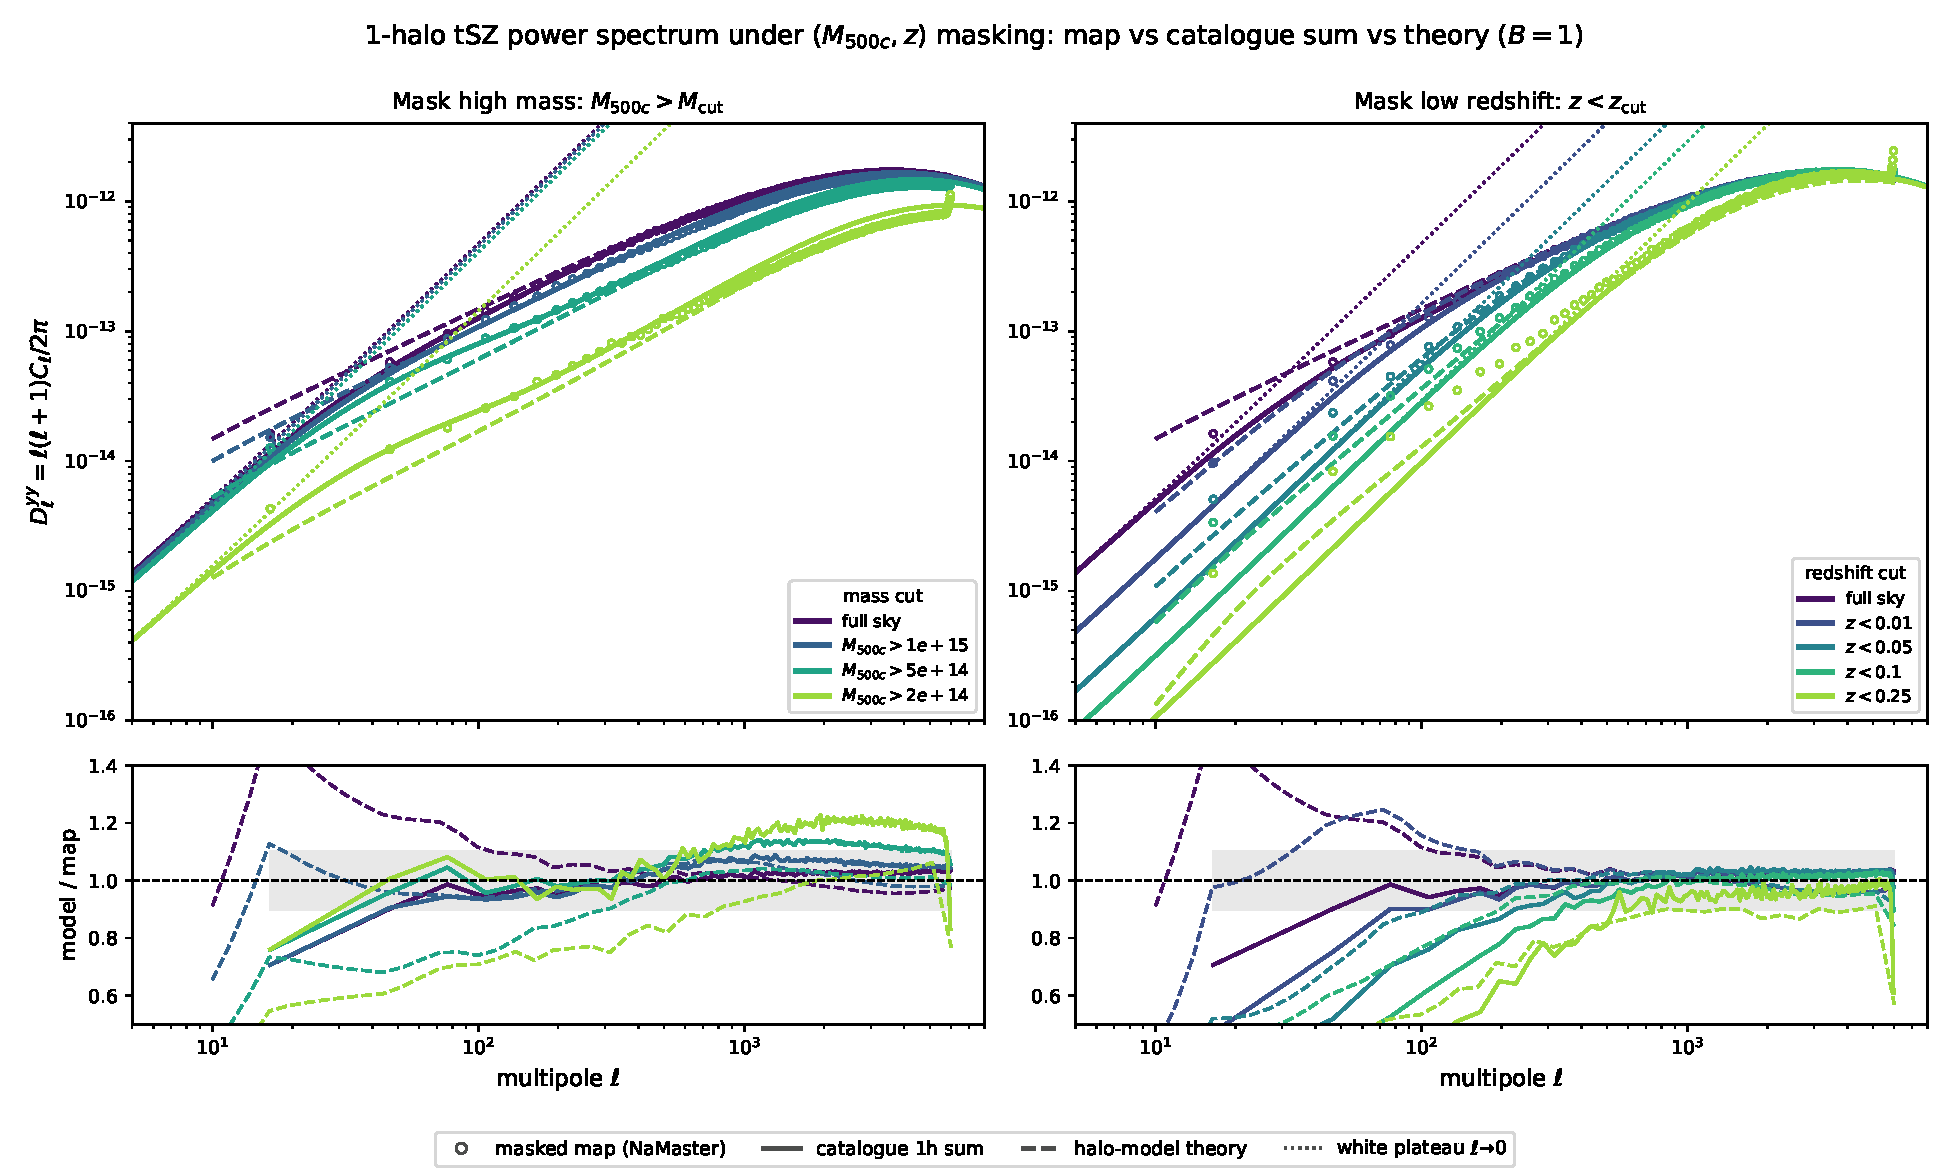
\includegraphics[width=0.95\linewidth]{flamingo_mz_masked_ps.pdf}
    \caption{\label{fig:flamingo_mz}%
    L2p8\_m9 tSZ power spectrum under direct $(M_{500\mathrm{c}}, z)$ masking; styles as in Fig.~\ref{fig:flamingo_snr}.
    Left: removing haloes above a mass cut ($M_{\mathrm{cut}} = 10^{15}, 5\times 10^{14}, 2\times 10^{14}\, M_\odot$) suppresses the spectrum near its peak (the theory $D_{3000}$ falls from $1.6 \times 10^{-12}$ to $6.3 \times 10^{-13}$ for $M > 2\times10^{14}\, M_\odot$).
    Right: removing haloes below a redshift cut ($z_{\mathrm{cut}} = 0.01, 0.05, 0.1, 0.25$) suppresses the largest angular scales sourced by nearby clusters; the white plateau falls by a factor of $48$ for $z < 0.25$.
    Since the selection is a deterministic top-hat in $(M, z)$, the halo-model mask is exact and no completeness modelling enters.}
\end{figure*}

SNR selection mixes mass, redshift, and scatter.
To separate these axes we repeated the exercise with deterministic top-hat masks directly in $(M_{500\mathrm{c}}, z)$ (Fig.~\ref{fig:flamingo_mz}).
The two progressions dissect the spectrum into its halo populations.
Masking the most massive haloes removes power at intermediate and high multipoles: the objects are rare (little sky is lost) but individually bright, and dropping all haloes with $M_{500\mathrm{c}} > 2 \times 10^{14}\, M_\odot$ halves the spectrum at its peak.
Masking the lowest redshifts instead removes the largest angular scales, since nearby haloes subtend the largest $\theta_{500}$; the $z < 0.25$ cut suppresses the white plateau by a factor of $48$ while leaving the high-$\ell$ shape comparatively intact.
The halo-model theory with the same top-hat masks tracks the masked map across all cuts, and the growing gap between the catalogue sum and the map at low $\ell$ (catalogue-to-map medians rising from $1.03$ full sky to $1.19$ for $M > 2\times 10^{14}\, M_\odot$) is quantitatively accounted for by the two-halo term, which becomes relatively more important once the dominant one-halo objects are gone.

\subsection{Progressive masking of a single sky and feedback response}
\label{sec:flamingo_l1m9}

\begin{figure}[t]
    \centering
    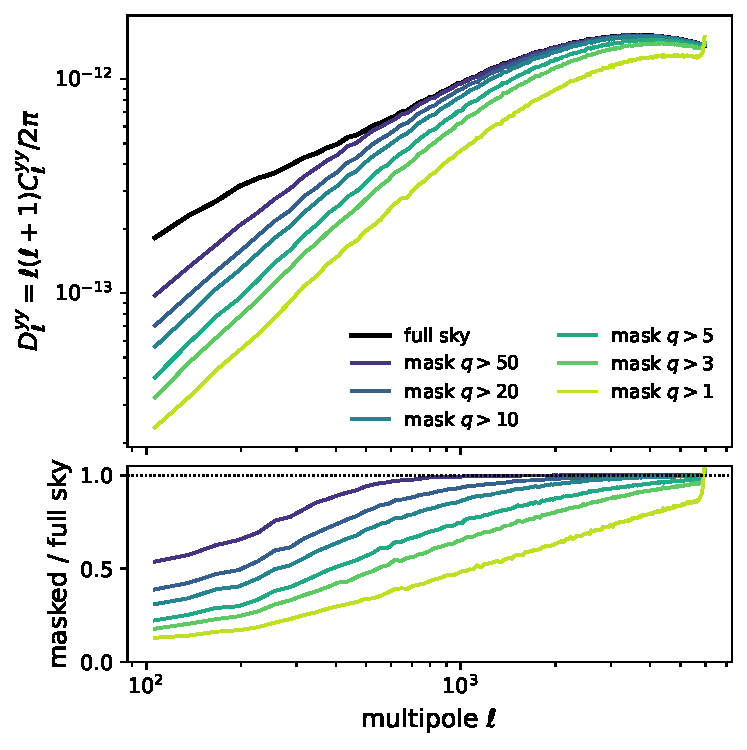
\includegraphics[width=\linewidth]{l1m9_progressive_masking.pdf}
    \caption{\label{fig:l1m9_masking}%
    Progressive SNR masking of the fiducial L1\_m9 sky ($B = 1.35$ selection; thresholds $q_{\mathrm{cat}} = 50$ to $1$).
    Top: masked bandpowers; bottom: ratio to the full-sky spectrum.
    The suppression is strongly scale-dependent: at $q_{\mathrm{cat}} = 5$ the masked spectrum retains $25$ per cent of the full-sky power at $\ell \simeq 140$ but $93$ per cent at $\ell = 3000$.
    The multipole at which the ratio recovers towards unity moves to higher $\ell$ as the threshold deepens, tracking the angular size of the faintest masked population.}
\end{figure}

The L1\_m9 box provides a single sky observed under nine feedback prescriptions, and a finer ladder of thresholds ($q_{\mathrm{cat}} = 50, 20, 10, 5, 3, 1$; the fiducial catalogue contains $4$, $49$, $217$, $1088$, $2888$, and $17\,730$ detections respectively).
Figure~\ref{fig:l1m9_masking} shows the fiducial spectrum under progressive masking.
The scale dependence of the suppression is the cleanest statement of which populations source which multipoles: masking at $q_{\mathrm{cat}} = 5$ removes three quarters of the power at $\ell \simeq 140$ but only $7$ per cent at $\ell = 3000$, and even the extreme $q_{\mathrm{cat}} = 1$ cut ($f_{\mathrm{sky}} = 0.72$) leaves $73$ per cent of the $\ell = 3000$ power in place.
The high-$\ell$ spectrum is therefore sourced overwhelmingly by haloes below any plausible detection threshold, while the low-$\ell$ spectrum is a shot-noise-like signal from the handful of giants; the two regimes respond to masking almost independently.

\begin{figure*}[t]
    \centering
    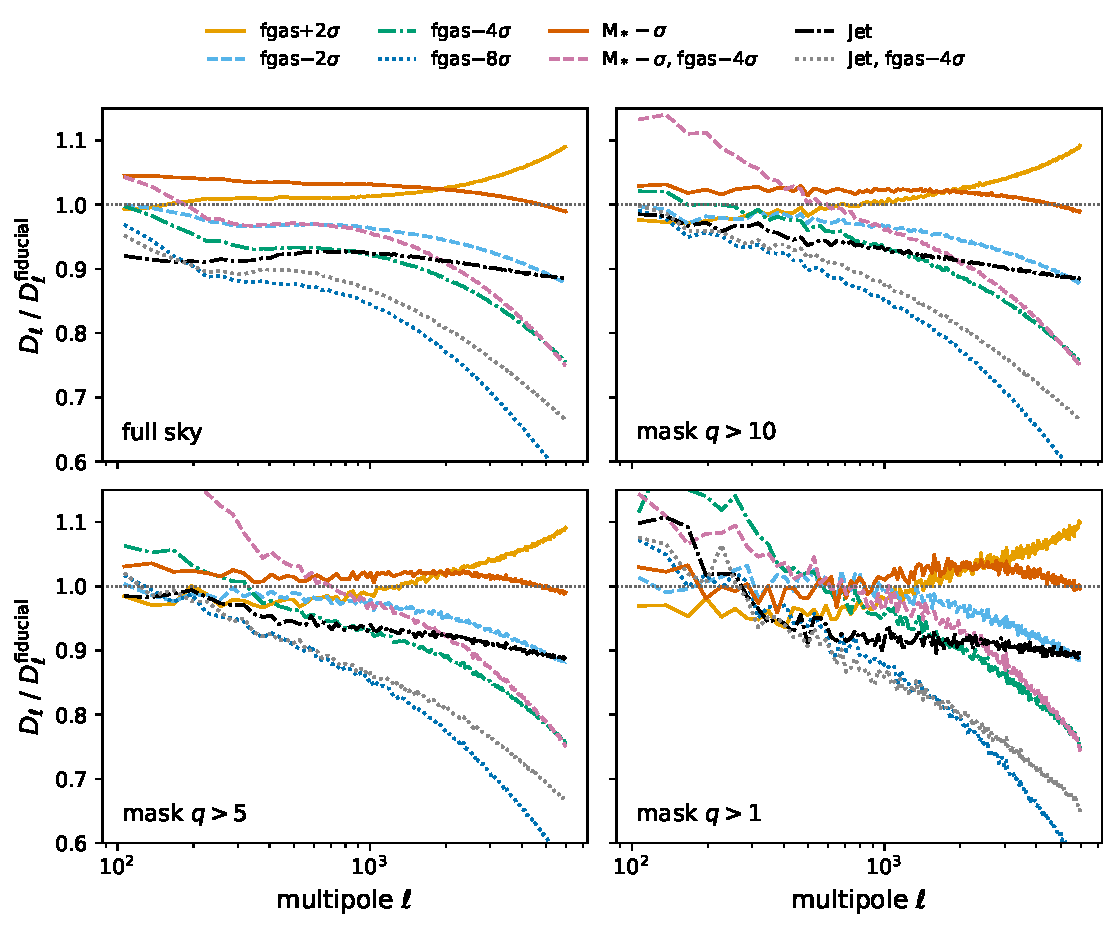
\includegraphics[width=0.9\linewidth]{l1m9_feedback_ratio.pdf}
    \caption{\label{fig:l1m9_feedback}%
    Ratio of the tSZ power spectrum in each L1\_m9 feedback variant to the fiducial run, for the full sky and after masking at $q_{\mathrm{cat}} = 10$, $5$, and $1$.
    Line colour and style identify the variant (legend on top).
    The fractional feedback imprint survives masking essentially unchanged at high multipoles (relative full range $0.33$ at $\ell = 3000$ both before and after the $q_{\mathrm{cat}} = 5$ mask), while the low-$\ell$ ratios become noisier as the surviving power is dominated by ever fewer objects.}
\end{figure*}

Figure~\ref{fig:l1m9_feedback} addresses the third question: does removing the giants also remove the astrophysics?
It does not.
At $\ell = 3000$ the full range across the nine variants is $33$ per cent of the fiducial power on the full sky (from $+4$ per cent for $\mathrm{fgas}{+}2\sigma$ to $-29$ per cent for $\mathrm{fgas}{-}8\sigma$), and the same $33$ per cent after masking at $q_{\mathrm{cat}} = 5$; at $\ell \simeq 300$ the range is $15$ per cent full sky versus $17$ per cent masked.
The feedback imprint on the tSZ spectrum is carried by the abundant low-mass, higher-redshift population, precisely the haloes that survive the mask, while the masked giants contribute rare-object noise rather than feedback information.
Masking therefore delivers a spectrum that is simultaneously more Gaussian (Sec.~\ref{sec:gaussianity}), decorrelated from the counts (next subsection), and undiminished as a probe of baryonic feedback.
We note that the variant ordering is coherent across thresholds: reducing cluster gas fractions or introducing jet feedback lowers the spectrum at all masking levels, consistent with the full-sky feedback phenomenology of FLAMINGO \citep{Schaye2023,McCarthy2023}.

\subsection{Masking decorrelates counts and power spectrum}
\label{sec:flamingo_decorr}

\begin{figure*}[t]
    \centering
    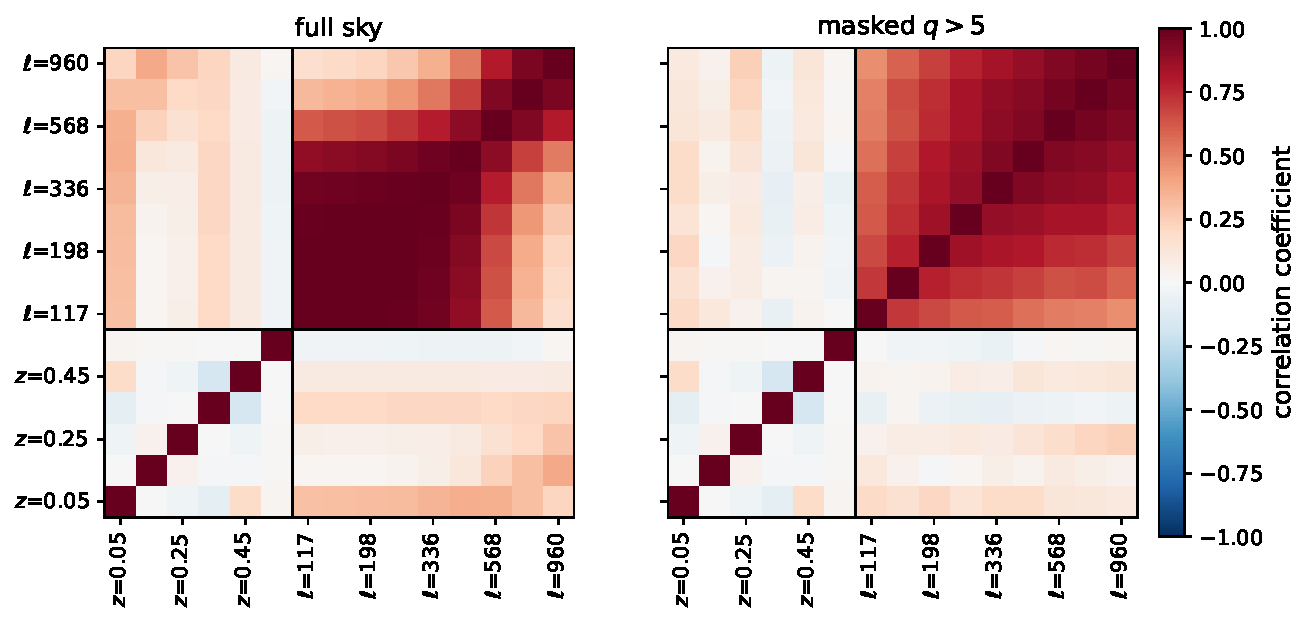
\includegraphics[width=0.82\linewidth]{l1m9_cnc_ps_corrmat.pdf}
    \caption{\label{fig:corrmat}%
    Joint correlation matrix of the data vector $[N_{\mathrm{cl}}(z),\ C_\ell]$ estimated from $192$ HEALPix $N_{\mathrm{side}} = 4$ patches ($\sim 215\,\mathrm{deg}^2$ each) of the fiducial L1\_m9 sky, for the full-sky spectrum (left) and the masked $q > 5$ spectrum (right).
    The redshift bins cover $0.005 < z < 0.6$ (counts at $q > 5$); the nine bandpowers span $\ell_{\mathrm{eff}} = 117$ to $960$.
    Masking suppresses both the strong low-$\ell$ bandpower correlations (upper-right block) and the counts-bandpower cross block, whose mean falls from $+0.135$ to $+0.057$.}
\end{figure*}

\begin{figure}[t]
    \centering
    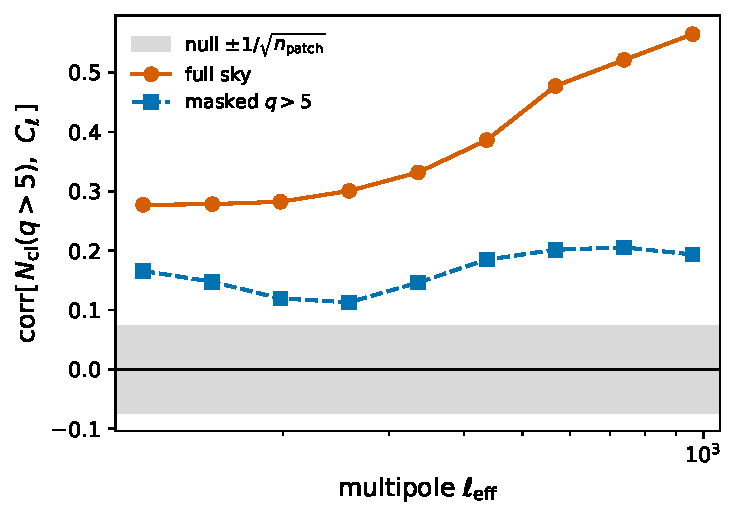
\includegraphics[width=\linewidth]{l1m9_cross_corr_vs_ell.pdf}
    \caption{\label{fig:crosscorr}%
    Correlation between the total cluster count $N_{\mathrm{cl}}(q > 5)$ and each bandpower across the $192$ L1\_m9 patches.
    The grey band is the null expectation $\pm 1/\sqrt{n_{\mathrm{patch}}}$.
    Masking reduces the mean correlation from $+0.38$ (rising to $+0.56$ at $\ell_{\mathrm{eff}} = 960$) to $+0.16$; the residual is patch-level large-scale-structure coupling through the two-halo term, and is absent ($+0.016$) in an unclustered painted Monte Carlo with the same selection.}
\end{figure}

The factorised likelihood of Eq.~\eqref{eq:joint} assumes that the masked spectrum and the counts are effectively independent.
Following the covariance analysis of \citet{Hurier2017}, we tested this assumption empirically by resampling the fiducial L1\_m9 sky in $192$ HEALPix $N_{\mathrm{side}} = 4$ patches and measuring the joint correlation matrix of the binned counts and the bandpowers (Figs.~\ref{fig:corrmat} and \ref{fig:crosscorr}).
Without masking, the counts correlate with every bandpower at the $+0.28$ to $+0.56$ level: the same massive clusters that enter the catalogue dominate the patch-to-patch scatter of the spectrum.
Masking at the catalogue threshold removes exactly those objects, and the mean counts-bandpower correlation drops from $+0.38$ to $+0.16$.
The residual correlation is not a masking failure but genuine large-scale-structure covariance: patches that are overdense host both more clusters and more unresolved power through the two-halo term.
A painted Monte Carlo with Poisson-sampled (unclustered) haloes and the same selection shows a null cross-correlation of $+0.016$, confirming this interpretation.
The patch ensemble itself is validated by two anchors: the summed patch counts reproduce the full-sky catalogue exactly ($N(q>5) = 1088$), and the patch-mean bandpowers agree with the full-map NaMaster measurements to between $0.999$ and $1.032$ (full sky) and $0.982$ and $1.009$ (masked) across the nine bins.
For \textit{Planck}-like analyses the residual $+0.16$ coupling is negligible compared with the noise; for future low-noise surveys it can be modelled with a super-sample term or measured with exactly this patch construction.

%==============================================================================
\section{Discussion}
\label{sec:discussion}
%==============================================================================

The two stages of this study are deliberately complementary.
On synthetic skies, where the data generation matches the likelihood, masking converts the tSZ bandpower distribution into a Gaussian in every bin and the joint CNC plus masked-tSZ analysis is both tighter (factors of $1.4$ to $5$ over single probes) and less biased than the combination with the full-sky spectrum.
On FLAMINGO, where the intracluster medium is simulated rather than painted, the same masking operation behaves as the formalism predicts: the surviving spectrum is tracked by the completeness-weighted halo model and by a model-free catalogue summation, the counts decouple from the surviving bandpowers, and the feedback information carried by the unresolved population is preserved.

Three limitations bound the present results.
First, the foreground sector: the synthetic analysis shows that with a fixed template basis the joint constraints are limited by foreground residuals, with the most tSZ-degenerate template absorbing a $3.8\sigma$ amplitude bias.
Any application to real data inherits this limit and will require either a physical foreground model or external priors on the mass bias $B$.
Second, we did not run parameter inference on the FLAMINGO skies.
Beyond the weak constraining power of a single realisation, the halo mass function of FLAMINGO differs from the Tinker08 calibration used in our forward model at a level that biases $S_8$ in counts-only fits; a joint FLAMINGO inference is only meaningful once an emulated FLAMINGO mass function replaces Tinker08, which we leave to future work.
Third, the two FLAMINGO analyses use different selection conventions ($B = 1$ with measured Compton parameters on L2p8\_m9; parametric $B = 1.35$ amplitudes on L1\_m9).
Each is internally consistent between mask and catalogue, which is what the method requires, but a real-survey application should derive both from the same calibrated scaling relation.

The progressive-masking decomposition of Sec.~\ref{sec:flamingo} also has a diagnostic value independent of the joint likelihood.
Because the mass and redshift cuts move the spectrum in characteristically different ways (mass cuts suppress the peak; redshift cuts suppress the largest scales), measured masked spectra at several thresholds constrain the mass and redshift decomposition of the tSZ background directly, and the threshold ladder of Fig.~\ref{fig:l1m9_masking} is in effect a tomography of the halo population in signal-to-noise.
The persistence of the feedback imprint under masking (Fig.~\ref{fig:l1m9_feedback}) is particularly relevant for upcoming low-noise surveys \citep{SimonsObservatory:2018koc,CMB-S4:2022ght}, for which the unresolved tSZ background at $\ell \gtrsim 2000$ is a target observable for constraining AGN feedback: our results show that removing the resolved clusters, which those surveys will do anyway for their counts analyses, does not degrade that target.

%==============================================================================
\section{Conclusions}
\label{sec:conclusions}
%==============================================================================

We have presented a self-consistent joint analysis of the tSZ power spectrum and cluster number counts in which the clusters detected above a threshold $q_{\mathrm{cat}}$ are masked from the map and counted in the catalogue, so the two probes act on disjoint halo populations.
Our main findings are as follows.
\begin{enumerate}
    \item On synthetic \textit{Planck}-like skies, masking renders the binned bandpower distribution statistically Gaussian in every multipole bin, whereas the full-sky distribution is strongly skewed at $\ell \lesssim 100$; the Gaussian power spectrum likelihood is then valid on all scales.
    \item The joint CNC plus masked-tSZ analysis reaches $\sigma(\Omega_{\mathrm{m}}) = 0.008$, $\sigma(\sigma_8) = 0.009$, and $\sigma(F) = 0.003$ in the signal-only case, factors of $1.4$ to $5$ tighter than any single probe, and retains factor $2$ to $4$ gains under foreground contamination; the analysis is then limited by foreground-residual modelling, which biases the most tSZ-degenerate template amplitude by $+3.8\sigma$.
    \item Applied to the FLAMINGO simulations, progressive masking reveals a strongly scale-dependent decomposition of the tSZ spectrum: at $q_{\mathrm{cat}} = 5$ the mask removes $75$ per cent of the power at $\ell \simeq 140$ but only $7$ per cent at $\ell = 3000$.
    Mass cuts suppress the spectrum near its peak while redshift cuts suppress the largest scales, and both the masked map and a model-free catalogue summation are reproduced by the completeness-weighted halo model (to a median of $3$ per cent on the full sky).
    \item Masking decorrelates the two probes on the simulated sky, reducing the mean counts-bandpower correlation from $+0.38$ to $+0.16$ across $192$ patches, with the residual attributable to two-halo super-sample coupling; this empirically supports the factorised joint likelihood.
    \item Masking preserves the fractional imprint of the FLAMINGO feedback variants on the spectrum ($33$ per cent full range at $\ell = 3000$ before and after the $q_{\mathrm{cat}} = 5$ mask): the astrophysical information in the tSZ background resides in the unresolved population, not in the masked giants.
\end{enumerate}
Together these results establish massive-cluster masking as the natural interface between cluster number counts and the tSZ power spectrum: it removes the double counting, the non-Gaussianity, and the cross-covariance in one operation, at no cost in astrophysical sensitivity.
The next steps are the replacement of the fixed foreground templates with a physical model, an emulated FLAMINGO mass function to enable end-to-end joint inference on the hydrodynamical skies, and the application to \textit{Planck} data.

%==============================================================================
\begin{acknowledgments}
We thank the FLAMINGO collaboration for making the simulation outputs available.
% [Funding and computing acknowledgments to be completed.]
\end{acknowledgments}
%==============================================================================

\bibliography{refs}

\end{document}
